\documentclass[a4paper,13pt]{report}
\usepackage[latin1]{inputenc}
\usepackage[english]{babel}
\usepackage[pdftex]{graphicx} 
\usepackage{sidecap}
\usepackage{pdfpages}
\usepackage{fancyvrb}
\usepackage{floatrow}
\usepackage{float}
\usepackage[section]{placeins}
\usepackage{fancyvrb}
% \usepackage{bera}% optional: just to have a nice mono-spaced font
\usepackage{xcolor}
\usepackage{listings}
\bibliographystyle{unsrt}

\colorlet{punct}{red!60!black}
\definecolor{background}{HTML}{EEEEEE}
\definecolor{delim}{RGB}{20,105,176}
\colorlet{numb}{magenta!60!black}

\lstdefinelanguage{JSON}{
    basicstyle=\normalfont\ttfamily,
    numbers=left,
    numberstyle=\scriptsize,
    stepnumber=1,
    numbersep=8pt,
    showstringspaces=false,
    breaklines=true,
    frame=lines,
    backgroundcolor=\color{background},
    literate=
     *{0}{{{\color{numb}0}}}{1}
      {1}{{{\color{numb}1}}}{1}
      {2}{{{\color{numb}2}}}{1}
      {3}{{{\color{numb}3}}}{1}
      {4}{{{\color{numb}4}}}{1}
      {5}{{{\color{numb}5}}}{1}
      {6}{{{\color{numb}6}}}{1}
      {7}{{{\color{numb}7}}}{1}
      {8}{{{\color{numb}8}}}{1}
      {9}{{{\color{numb}9}}}{1}
      {:}{{{\color{punct}{:}}}}{1}
      {,}{{{\color{punct}{,}}}}{1}
      {\{}{{{\color{delim}{\{}}}}{1}
      {\}}{{{\color{delim}{\}}}}}{1}
      {[}{{{\color{delim}{[}}}}{1}
      {]}{{{\color{delim}{]}}}}{1},
}
\bibliographystyle{unsrt}
\begin{document}

\begin{titlepage}
\begin{center}

\includegraphics[width=5cm]{EURECOM_logo_quadri}
\\[3cm]
\textbf{\Huge{Building NERD dashboard}}
\\[2cm]
\textbf{\textsc{\LARGE{Semester Project Report}}}
\\[0.5cm]
\LARGE{Chillari Paolo}
\\
\large{Fall 2011}
\\[8cm]
\columnsep3cm
\begin{tabular}{p{8cm} p{8.5cm}}
\small{\textbf{Supervisors:}\newline
Rapha\"el Troncy\newline
Giuseppe Rizzo} 
&\small{\textbf{EURECOM\newline Multimedia Department}}
\end{tabular}
\end{center}
\end{titlepage}

 \tableofcontents

\chapter{Introduction}
Dashboards have become the de facto face of performance management applications and are increasingly used in business intelligence (BI). The world of web is becoming itself the world of big data, but frequently it's hard to give meaning and extract useful information from this huge amount of bytes. How this information are presented to administrators is critically important and make data understandable to human eyes.\newline

There are zettabytes of data in the world today and companies, associations, research labs are drowning in information. Dashboards place the data the this entities need in a visual, easy-to-understand format. The ability to see the data that you need and when you need it gives you the ability to quickly understand the current situation at any given point in time. Rather than digging through databases, logs files, spreadsheet you can consult your dashboard for a quick insight.\newline

A dashboard democratizes access to big data, so that anyone  can have the right information at his fingertips.

Dashboard has become integral and substantive part of web application panorama giving privates, companies, IT service providers, etc the ability to handle their business efficiently. Dashboard, as a matter of fact, could achieve different goals, from strategic to analytical or operational requirements.\newline
The main focus of this project is on Administration Dashboards, where admins can have a full overview of what is happening on their platform. The dashboard summarizes in one single location all the information that an administrator need: from user's information to how many visits, page-views and other detailed information about the platform. In some cases, like for the Nerd Application, should provide a common interface for interacting with data stored by the entire system.

\chapter{Similar projects}

The web panorama is full of great example of dashboard and how they became the pivot of huge businesses.
\section{3scale}
3scale is a management solutions for developers and companies to securely distribute, control, manage, operate and monetize their API. His API management platform is Plug and Play, configurable, flexible and scalable bringing API providers an unparalleled level of ownership, control and configuration to ensure QoS, SLA and a great user experience.
3Scale exposes a Dashboard to monitor the API usage, in order to give the developer a full overview and control on the usage of his APIs.
3scale shares with NERD some key point and therefore it  represents a good case of study.

The main features:
\begin{itemize}
\item \textbf{Usage}\newline
 3Scale exposes a time-line chart to show the total usage of the APIs. The timeline is navigable in time and the dashboard admin could filter data by  metrics or API methods.

\item  \textbf{Top Applications}\newline
As for the usage, we have a another time-line chart. One of the cool features of 3Scale is that the developers has a full overview of the usage of his APIs for every application that is using it.It's possible to choose metrics and methods for our statistics.

\item \textbf{Daily and weekly usage}\newline
 3Scale dashboard also allow to aggregate by hour of the day and day of the week: take under control the load in different time of the day or different days of the week become easier.


\item \textbf{Other features}\newline
As the others main dashboard services, 3Scale allows to define alerts, in order to give the developer updates about data that he cares most.
\end{itemize}

\chapter{Dashboard Design Study}
\section{Framing the Dashboard - Structure}
This section offers ideas about big-picture elements and building blocks to be used to construct a dashboard. \newline The building blocks can be broken into four categories.
\subsection{Form}
It's important to select the form that fits the needs of the situation.
The goal is to understandably show critical information and make it available when the audience needs it.
\begin{itemize}
\item  \textbf{Timeliness}\newline
Frequency of  data update
According to the most popular dashboard and, first of all, to Google Analytics, data's update follows two main patterns. In the first one data  is displayed and updated in response to a request made directly by the administrator by the UI while the second one (commonly in parallel) is to have data  displayed in real time. The administrator could see what is happening on the framework in that moment. Concerning Nerd Dashboard the administrator could have, for example, a global overview of the usage of the rest APIs, how much users are currently using it, from where, what are the REST methods and entities accessed.
\item \textbf{Aesthetic}\newline
For the Nerd framework this could be not the most urgent and important feature to achieve, but for a personal point of view and according to the Juiceanalytics article \cite{Juice} a good aesthetic reflects a good usability and makes the accessibility to  data easier.
As a matter of facts Google Analytics in the last years put huge efforts to change and improve the UI and aesthetic of the dashboard.
\item\textbf{Mobility}\newline
Since administrators of Nerd has to travel all around the world, the chance to access data on the go is an important feature. Administrators need to have data accessible from everywhere using laptops but also tablets and smartphone. An overview of the dashboard should be accessible in every moment they need to.
\item \textbf{Connectivity}\newline
Depending on the amount of data that has to be accessed and how the administrator has to filter and parametrize data, it's possible to follow different patterns. 
In order to achieve the real time features the backend module that handle the dashboard has to talk directly with data-source.
\item \textbf{Data detail}\newline
The administrator has to access data in detail, dive into all the information stored on the database. But this data has to be presented in the right way in order: the page has not to be a heap of meaningless numbers.
\item \textbf{Data density}\newline
 How much information rich will views of the data be? The best structured way to achieve a balance data density is to reveal information as the administrators express interest. In other words, don't bombard the admins with all the information at once, using levels of increasing detail from 
\item \textbf{Interactivity}\newline
The Nerd admins have to actively interact with the dashboard in order to organize, filter, define metrics on the data he needs. A great dashboard requires to be customizable and, especially for Nerd, the admins have to fully interact with the data that comes from it.
\item \textbf{Collaboration}\newline
There is a team working on the network so it could be useful to cooperate on the framework. But I think that for Nerd the dashboard could not be the right tool to achieve this collaboration, there are betters tools that are born to handle collaboration in the field of Computer Science Development and Research. 
I see this tool more for a business or strictly administration dashboards.
\end{itemize}
\subsection{Structure}
\emph{``Dashboard content must be organized in a way that reflects the nature of the information and that supports efficient and meaningful monitoring. Information cannot be placed just anywhere on the dashboard.''}\newline
\emph{``Important items should often appear larger, thus more visually prominent than less important items''}

\begin{itemize}
    \item \textbf{Flow}\newline
    A flow-based structure emphasizes a sequence of events or actions across time
    \item \textbf{Relationship}\newline
    The structure of a dashboard can also emphasize the relationships between entities or measures. These relationships or connections may be mathematical, geographical or functional.
    \item \textbf{Grouping}\newline
    The structure of last resort is to group related information into categories or a hierarchy. The structure of last resort is to group related information into categories or a hierarchy
\end{itemize}
\subsection{Design Principles}
Few core design goals that as to be reminded as you get closer to start sketching your application: is quite difficult to straightly follow simultaneously all these key design principle, instead it's better to pick one or two with higher priority to help stay focused.
\begin{itemize}
    \item \textbf{Compactness/Modularity}\newline
    Dashboard could become large and unwieldy, especially when it tries to give a comprehensive view of huge business that could be, in their fullness, various and heterogeneous. Compactness is the property that a design can fit inside a human being's head.
    A dashboard can be broken into bite-sized pieces, each built around a key question in order to be organized and give to the administration a more organized and ordained view.
    \item \textbf{Gradual reveal}\newline
    Reveal information as the dashboard user expresses interest. Don't bombard the administrator with all the information at once (use levels of increasing details)
    \item \textbf{Customizable}\newline   
    Allow users to customize the dashboard (defining the scope). 
    Does the dashboard let the admins save a view of data that they have configured? \newline
    Does it offers easy ways to tag or highlight things that are important to them?
    \item \textbf{Explanation before information}\newline
    Dashboards need to give the context and explanation to understand new and unfamiliar events.Letting the data speak for itself can be a recipe for misinterpretation and confusion.
\end{itemize}

\subsection{Functionalities}
\begin{itemize}
\item \textbf{Filters}\newline
Allow users to define the scope of the data in the dashboard to reflect their needs. Filters can either be global (refining scope for the entire dashboard) or local(refining scope for a specific chart or metric or view).

\item \textbf{Comparison}\newline
Ability to see two or more subsets of the data side-by-side. A line chart, for example, may let the the Admin view two geographic regions as separate lines or in the same chart lines of different colors for the same source of data with different filters applied

\item \textbf{Alerts}\newline
Highlight information based on pre-defined criteria. Alerts may be activated when a metric goes outside of a particular threshold.  The administrator could define alerts for instance when a threshold for a first class object is reached, based on some predefined filters and more in general on whatever could be a matter of statistics both in absolute and relative value.

\item \textbf{Export / print}\newline
The  admin should have the ability to export data out of the dashboard in different formats. In details, should be possible to not only export all the data available but the exported data should reflect filters, metrics, parameters that the administrator could defined: for instance every personalized widget should be exportable as a chart or as a table of data.
\end{itemize}

\section{Information Design}
In this last part we provide practical tips for putting information on the page in a way that communicates effectively to our audience. How data is presented is a primary goal and it strongly affects the final result. Best practices for designing a clear, aesthetically-pleasing page are key factors.\newline
A clear and simple interface is the primary goal and deals with limiting visual clutter to allow the user to easily navigate and understand the content on th page.

\begin{itemize}
\item \textbf{Organizing the page: } information could not be just arranged on the page without order, semantics and taking into account where people looks first, where information should be to capture user's attention.
Moreover a \"grid system\" approach brings order and coherence into the page. Finally white spaces can be used to delineate sections or help users see groupings of content in a dashboard. Using white space means sacrificing one extra chart or metric, but it can make a huge difference in user comprehension.

\item \textbf{Colors:}
Appropriate use of color requires restraint. In our dashboard designs, we typically start by using only gray and then add colors where it conveys useful information.
Colors bring meaning: they can draw your eye to what is important and tie together similar things.

\item \textbf{Typography: }it includes everything from choosing a typeface to picking the right point size, kerning, tracking and leading.
Simple font framework:
\begin{itemize}                                    
\item Body text is clean, readable content
\item Headers separate and name major sections of the work                                                       
\item Notes describe additional things the reader should be aware of. These should fade into the background unless we call attention to them.
\item Emphasis text is what we want our reader to pay particular attention to.   
\end{itemize}
\end{itemize}

\chapter{Designing NERD dashboard}
\section{Functionalities}
    We already talk about the aims of the Web Application and now we can dive deeper in the functionalities exposed.
    Firstly we have a section `` Users '' where we have statistics on the number of the new users registered on nerd.eurecom.com. We can easily navigate in time on the y-axis and aggregate data by day, week, month and year. Moreover the timeline widget allows the admins to customize the graph: through a handy modal he can add filters to data choosing dimensions, operators and values for the filters. In Addition he has the possibility to add lines to the graph, with their own filters, in order to allow the user to compare statistics with different filters.
    Furthermore in this section we can find pie charts that allows us to have an overview of the users group by language, country and language.
    We have then an other section were we can find statistics on entities extracted by the framework and more specifically on the entity types extracted: as for the user we can navigate data through the timeline widget, defining filters and adding new lines. Pie charts allow to see how different Language Processing Services aggregate entities, showing the ratio between different NERD Core Classes from different services.
    Lastly the administration can monitor the usage of the APIs with information on the number of annotations.
    Nerd Dashboard also allows the profile administrations that have their own filters: the Web Application transparently saves charts settings for the administrators
   In this chapter we discuss the state of the art and the reasons that leads our architectural and development decisions.

\section{State of the art}
The web panorama is widely spread and choosing the right architecture having clear in mind the problems and goals of the project is critically important. 
The world of the web during the last years is surrounded by a whirlwind of change, one of which is the dramatical increase of adoption of Single Application Architecture.\newline

Most popular Web Application like Gmail, Google Maps, Google Drive, iCloud, GitHub, Hotmail and many others are common SPAs.
A SPA is an application that runs inside a browser (or in a ``compatible'' environment) and does not require page reloading during use. We can think of a SPA as a thick client that is loaded from a web server. 
SPAs are all about providing an outstanding user experience by trying to replicate a ``native'' environment in the browser , no page reloads, no extra wait time.

In order to fully understand this great shift we have to make a short overview of ``the classical Web Architecture''.
\subsection{Classical Web Architecture}
The Web is a two tiered architecture where the web browser displays the content and the Web Server is responsible to transfer information to the client.
This is not an exhaustive definition and to fully understand the web paradigm we have to dive into how this two entities interact with each other.
Most web applications use a server-templating model. This model relies on an application server that processes data and sends it out as HTML, which, in the end, is rendered on the client. When the user clicks a button or a link on that page, a HTTP POST or GET operation is sent to  the application server and a brand new HTML page is returned to the client browser to be rendered again.\newline
The main problems this architecture is facing today are:
\begin{itemize}
\item \textbf{Bad user experience: } Continuous page re-rendering has a negative impact on the user experience: network latency cannot be hidden from the user.
\item \textbf{Poor performance: } Unnecessary re-transmission of data occurs because completely reloads on each user interaction.
\item \textbf{Lack of offline support: }A web application is alive as long as there is a server connectivity. If the server connectivity drops, the web application is practically worthless.
\item \textbf{Sever overload: } The great part of the work is demanded to the server side. 
\end{itemize}

\begin{figure}[H]
  \centering
    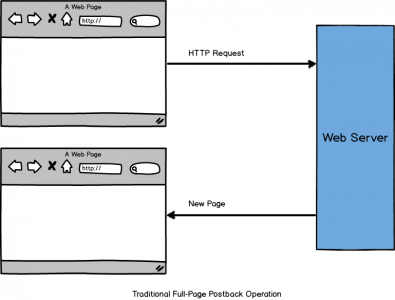
\includegraphics[width=0.7\textwidth]{pics/architecture}
\end{figure}

\subsection{Single Page Application Architecture}
 One of the main reason to choose SPA is because it offers a more-native-app-like experience to the user. As we already said this kind of experience it is hard to do with other approachess.
 Supporting rich interactions with multiple components on a page, means that those components have many more intermediate states and a server-side rendering is hard to implement for all the intermediate states - small view states do not map well to URLs.

Single page apps are distinguished by their ability to redraw any part of the UI without requiring a server roundtrip to retrieve HTML. This is achieved by separating the data from the presentation by having a model layer that handles information and a view layer that reads from the models.


This is the definition given by Wikipedia \cite{SPAWikipedia}:
\begin{quotation}
A single-page application (SPA), also known as single-page interface (SPI), is a web application or web site that fits on a single web page with the goal of providing a more fluid user experience akin to a desktop application.
\end{quotation}


As well as being an evolution in Web design, SPA signals a much wider trend in the Web as a whole a separation of the functional layer as an API and the presentation layer in the form of the App (HTML5 or native):

The Single Page Architecture in parallel to the API Model is much more flexible than a HTML heavy page. The underlying API can be used to power a multitude of different front ends for different contexts, form factors and device types. Once the API is in-place, it can be used to serve multiple audience with different needs. \newline
\begin{quotation}
Single Page Apps arguably represent the final step in the unbundling of Web technology which started by separating out formatting from content (CSS), progressed to flexibility in structure (XML and XSLT), moved to disconnecting the page model from server calls (AJAX) and now unbundles the page structure from application navigation. This is a profound change in the way the Web works.
\end{quotation}
\begin{flushright}
from Steven Willmot - 3Scale CEO\cite{appification}
\end{flushright}
The potential for Single Page Apps arguably is that they can provide an experience very much analogous to native mobile and desktop apps anywhere where a web-browser with Javascript can be executed.

The pros of a SAP are :
\begin{itemize}
    \item
        \textbf{API oriented architecture: } Basically, it's just a deviation of classical `Server-client'', where we have server that provides an API and where client is a browser. Thus we have a much more modularized architecture: defined the API interface client and server are fully independent, much more testable, easier to maintain and the servers can power more heterogeneous client applications.

    \item
    \textbf{It renders like a desktop application: } SPA has the ability to redraw any part of the UI without requiring a server round-trip to retrieve HTML.

    \item
    \textbf{It renders like a desktop application: }
    It responds like a desktop application: SPA minimizes the response time by moving working data and processing as much as possible from the server to the browser. It has the necessary data and business logic to make most decisions on client. Only data validation, authentication, authorization and permanent storage occur on the server.
    \item
    \textbf{It notifies users of its state, like a desktop application:  }
    when a SPA has to wait on a server, it will render a progress bar or a busy indicator to prevent the user from getting confused by the delay. Also, navigation between different areas is smooth and continuous. Compare this to a traditional website, where the user actually has to guess when the page is loaded and usable.
    \item
    \textbf{Can go offline: }
     unlike the traditional web application, a SPA can go offline if the connectivity to the server drops. When the connection is on again, it synchronizes the local data with the server. Just think of mobile devices and you'll know how useful this feature is.
    \item
    \textbf{It is instantly updated and distributed, like a website: }
     users don't need to take any action. All they need to do is reload the browser and it works.
    \item
    \textbf{It renders like a desktop application: }
     unlike most desktop applications, a SPA works on any operating system that provides a decent browser. This is mainly considered a developer benefit, but think of users who use many devices.
\end{itemize}


\chapter{The Server}
        It is frequently not easy to choose the right server-side technology and there is never a right answer: much depends on the goals, performance requirements, amount of effort you're willing to expend and other hundreds of sensible factors.
        For our personal goals we choose to adopt Nodejs.\newline
        NodeJs
    \section {Why Node.js ?}
        \begin{quotation}
        Node.js is a platform built on Chrome's JavaScript runtime for easily building fast, scalable network applications. Node.js uses an event-driven, non-blocking I/O model that makes it lightweight and efficient, perfect for data-intensive real-time applications that run across distributed devices.
        \end{quotation}
        \begin{flushright}
          from Node.js website \cite{node}
        \end{flushright}


        \begin{itemize}
            \item
            \textbf{Code can easily be migrated to and from the browser/server}\newline
            

            Apart from using the Google Web Toolkit, there is really no way you can avoid JavaScript in a modern web application. \newline

            Using Node, the algorithms and data structures that you build can in theory run both on the client and on the server. It's easy to build modules context free and play around with where they run. 

            \item
            \textbf{Consistently asynchronous}\newline
            

            Everything in Node is asynchronous. This is powerful as it allows incoming requests to \textbf{conceptually} spawn off a set of threads at the same time. In most other environments you need to think serially. Since JavaScript has closures, programming asynchronously is straight forward.

            \item
            \textbf{JavaScript is a dynamic language}\newline
            

            For many problems, the ability to load code and execute it dynamically can significantly simplify the design. You can store code/functions as first-class objects and execute them upon need.

            \item
                \textbf{Npm community}

                The node.js Community growth since its birth has been dramatically fast and after two years on npm you can find every module for your needs.
                The numbers of published modules can describe better how Node.js is changing the world of Open Source:

                \textbf{python}:  29,720 packages / 22 years = 1351 packages per year\newline

                \textbf{ruby}:      54,385 packages / 18 years =    3022 packages per year\newline

                \textbf{node.js}:  26,966 packages / 4 years =   6742 packages per year \newline

                        \item
            \textbf{Frameworks}

            A large variety of Web Frameworks are available for Node.js: they will tie everything together for you and will ensure each piece fits together with the others.
            In particular to build powerful and flexible APIS Express is the best choice.
            \begin{quote}
            Express is a minimal and flexible Node.js web application framework, providing a robust set of features for building single and multi-page, and hybrid web applications.
            \end{quote}
                    \begin{flushright}
          from expressjs.com  \cite{express}
        \end{flushright}


            With Express you can have full control over your application and it's easy and quick to create robust user-friendly API.

        \end{itemize}
    \section{API Description}
        The client as we already said communicates with the server through simple REST API.
        Basically NERD dashboard retrieves information about the three first class objects from the server through GET request on the resource with some query parameters to specify which data the server has to retrieve from the mySql database.
        GET and POST requests on the resource ``filter '' allows to retrieve and update the filters used to profile the administrator.

    % \textbf{REST API documentation}:

        \begin{tabular}[ht]{p{3cm}|p{10cm}}
          Resource & Description \\
          \hline
          GET  /users & Retrieves data of users registrations \\
          GET  /entities & Retrieves data about the NERD core classes extracted \\
          GET  /annotations & Retrieves data of users registrations \\
          \\
          \textbf{Parameters} &

            \begin{description}
            \item [type]: specifies the family data format according to the graph type.\newline
                        Possible values: `'time`' , `'groupBy`''\newline
            \item [timeAggregation]: if type is defined and equal to `'time`', it specifies the temporal aggregation of data \newline
            Possible values:  `'week`',`'month`' and `'year`'.\newline

            \item [filters]: if type is defined and equal to `'time`', it specifies an array of filters applied on data \newline
            Example values: [\{`'dimension:`'country'', `'operator'':`'='', `'value'':`'france''\}, \{`'dimension'':`'language'', `'operator'':`'='', `'value'':`'french''\}].\newline


            \item [groupBy]: if type is defined and equal to `'groupBy`', it defines  the dimensional aggregation of data\newline
            Example values: `'country`', `'language`'

            \end{description}
 
             \\
            
        \hline
        GET /filters & Retreives filters of the current administrator from the server \\\\
        \textbf{Parameters:} & \textbf{entity:} defines the resource on which the filter should be applied\newline
        Possible values: `'users`',`'annotations`' and `'entities`'
        \\
        \hline
        POST /filters & Allow to save filters on a defined entity for an authorized administrator.\\ \\
         \textbf{Parameters:} & Array of Object Filter: Obj{dimension: ,operator: ,value:}


        \end{tabular}
        \newline\newline
        \newline\newline
        \textbf{Return Values}

    Here we have an example of a returned value of the GET method on the resource users with parameters type='time' and timeAggregation='month'

    GET /users?type=time\&timeAggregator=month
    \begin{lstlisting}[language=JSON]
        [
  {
    "year": 2012,
    "month": 11,
    "number": 3
  },
  {
    "year": 2012,
    "month": 12,
    "number": 84
  },
  {
    "year": 2013,
    "month": 1,
    "number": 51
  },
  {
    "year": 2013,
    "month": 2,
    "number": 48
  },
  {
    "year": 2013,
    "month": 3,
    "number": 84
  },
  {
    "year": 2013,
    "month": 4,
    "number": 67
  },
  {
    "year": 2013,
    "month": 5,
    "number": 95
  },
  {
    "year": 2013,
    "month": 6,
    "number": 94
  },
  {
    "year": 2013,
    "month": 7,
    "number": 9
  }
]
    \end{lstlisting}
The return object is the same for the other GET methods on annotations and entities.

An other example for the return value of a GET method on the resource Filter:

GET /filters?entity=user
  \begin{lstlisting}[language=JSON]
    [{
            "id": 1,
            "filter": [
                [{
                    "dimension": "country",
                    "operator": "=",
                    "value": "France"
                    }
                ],
                [{
                    "dimension": "language",
                    "operator": "=",
                    "value": "Italian"
                    }
                ]
            ]
        }
    ]
  \end{lstlisting}
    \section{Architecture}
    The Server is composed by the main core module, where the Express application object is instantiated and where the routes are defined. 
    This module delegates the real work to three other modules, one for each resource. These modules are composed by two main methods: the first is in charge to handle the request concerning the timeline information while the second handles the request on dimensional aggregated data.
    These functions, using the query parameters parsed by express, dynamically construct queries to send to the Database Management System.
    As we can see from the picture belows, these modules don't make direct access to the storage: the access is made through a module that handles the connections pool and make the calls to the native Node.js mySql driver.

\begin{figure}[ht]
  \caption{Module Diagram.}
  \centering
    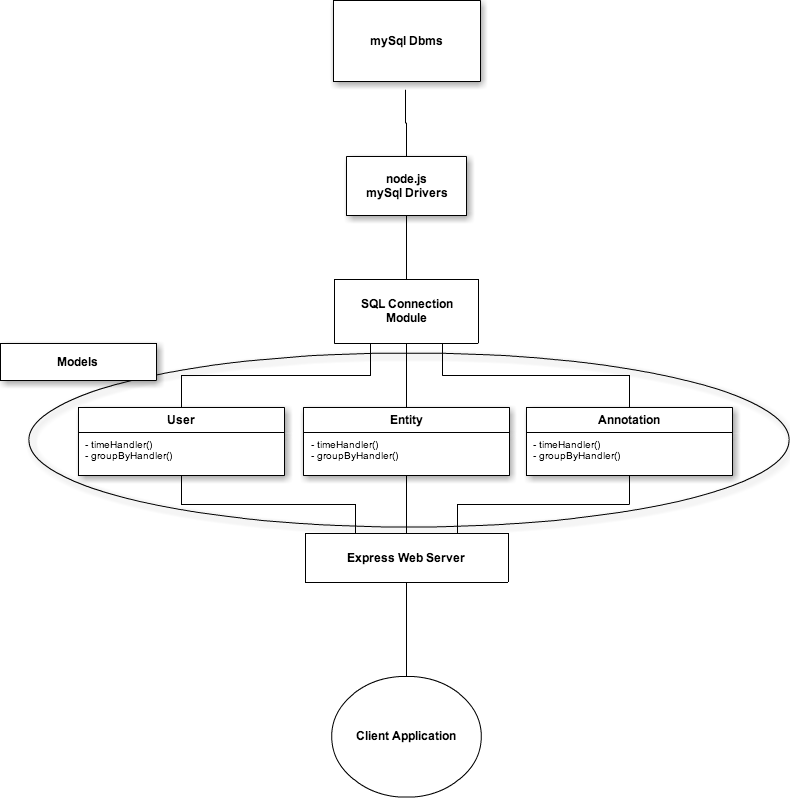
\includegraphics[height=1\textwidth]{pics/moduleChart}
\end{figure}

    \subsection{Round-trip request}
    In this section we have an overview on what are the steps in response to a client request to the server:
    \begin{enumerate}
        \item \textbf{Client request}\newline GET /users?type=time\&timeAggregator=day\&filters=[\{`'dimension'':`'country'', `'operator'':`'='', `'value'':`'france''\}] 
        \item \textbf{Express Server}\newline Express application parses the request, using Passport.js verifies if the request in authorized and finally delegates the user module to auto-generate the query.
        \item \textbf{User module}\newline This module auto-generates this query 
        \begin{lstlisting}[language=SQL]
        SELECT Year(registrationDate)  AS year, 
            Month(registrationDate) AS month, 
            Day(registrationDate)   AS day, 
            Count(iduser)         AS number 
        FROM   USER 
        WHERE  country = "france" 
        GROUP  BY Year(registrationDate), 
            Month(registrationDate), 
            Day(registrationDate), 
            country 
        \end{lstlisting}
        \item \textbf{SQL Connection Module}:
            This modules takes care to call the Native mySQL drivers and effectively retrieve the data from the database
        \item  \textbf{Express Server}
            Finally Express handle the response to the client creating the HTTP response.
    \end{enumerate}


    To handle the administration profiling, sessioning and authorization we used Passport.js which allows, in conjunction with Express Session to authorize users and create session easily.
\chapter{The Client}
 \section{Sketching}
Sketches are a crucial phase of our project and represents the start point of the dashboard design. The Dashboard Design Study described in Chapter 2 is the guideline and we tries to follow the best-practices.
Moreover, what strongly characterize our sketches is the purpose of build a fully responsive web app: 
\begin{quote} 
    Responsive Web Design (RWD) is a web design approach aimed at crafting sites to provide an optimal viewing experience-easy reading and navigation with a minimum of resizing, panning, and scrolling-across a wide range of devices (from desktop computer monitors to mobile phones).
\end{quote}

The world is changing fast and day by day, the number of devices, platforms, and browsers that need to work on the web grows dramatically. Responsive web design represents a fundamental shift in how we'll build websites for the decade to come.
Smartphones, tablets, Internet connected Tvs are becoming more and more popular bringing the problem of fragmentation to be put in the foreground.
In our project we handle this problem, starting from this first part: we decided to use an off canvas pattern for multi-device: this layout takes advantage of space off the screen to keep content or navigation hidden until either a larger screen size allows it to be visible or a user takes action to expose it.
\\[0.2cm]
\begin{figure}[H]
  \caption{Facebook example of Off Canvas Pattern .}
  \centering
    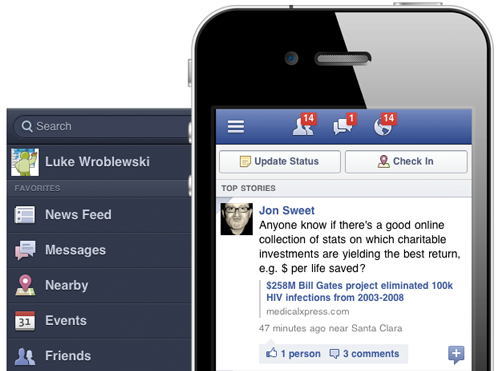
\includegraphics[width=0.7\textwidth]{pics/UISketches/offCanvas}
\end{figure}

The Off Canvas pattern is a interesting one because it doesn't force people to scroll long pages of content and navigation on small screens. Instead sections can be separated, labeled, and accessed when needed.


\subsection {Mobile UI}
It's becoming shared thinking that, to create a compelling and responsive website, it helps to focus first on smartphone users: start your design for small touchscreens and scale up from there. This can help ensure that a web application satisfies users on any device and loads quickly on any type of Internet connections.

% \begin{figure}
%   \centering
% \includegraphics[height=0.7\textwidth]%
%     {pics/UISketches/mobileSk1}% picture filename
%   \caption{ This sketch represents the view of one section of the dashboard, the contents fully occupies the page size, exploiting all the space and thus allowing the user to have charts and information larger on the page.}
% \end{figure}


\begin{figure}[H]
\floatbox[{\capbeside\thisfloatsetup{capbesideposition={left,top},capbesidewidth=4cm}}]{figure}[\FBwidth]
{\caption{This sketch represents the view of one section of the dashboard. Contents fully occupy the page, exploiting all the space allowing the user to have charts and information larger and more readable.}\label{fig:test}}
{\includegraphics[width=5cm]{pics/UISketches/mobileSk1}}
\end{figure}



% \begin{figure}
%   \centering
% \includegraphics[height=0.7\textwidth]%
%     {pics/UISketches/mobileSk2}% picture filename
%   \caption{ This sketch represents the step forward the interaction with the icon floated left on the top bar. The menu slides right and the content with him: now the space is optimized for displaying the sidebar and allowing the user to easily interact with the navigation items }
% \end{figure}


\begin{figure}[H]
\floatbox[{\capbeside\thisfloatsetup{capbesideposition={right,top},capbesidewidth=4cm}}]{figure}[\FBwidth]
{\caption{This sketch represents the step forward the interaction with the icon floated left on the top bar. The menu slides right and the content with him: now the space is optimized for displaying the sidebar and allowing the user to easily interact with the navigation items}\label{fig:test}}
{\includegraphics[width=5cm]{pics/UISketches/mobileSk2}}
\end{figure}

\begin{figure}[H]
\floatbox[{\capbeside\thisfloatsetup{capbesideposition={left,top},capbesidewidth=4cm}}]{figure}[\FBwidth]
{\caption{This sketch represents the interface to modify the options for a chart: everything goes on the background and the options panel occupies the majority of the page}\label{fig:test}}
{\includegraphics[width=5cm]{pics/UISketches/mobileSk3}}
\end{figure}


% \begin{figure}
%   \centering
% \includegraphics[height=0.7\textwidth]%
%     {pics/UISketches/mobileSk3}% picture filename
%   \caption{ This sketch represents the interface to modify the options for a chart: every thing goes on the background and the options panel occupies the majority of the page }
% \end{figure}


\subsection{ Tablet and Desktop UI  }

As suggested by the  the Off Canvas Pattern, shifting on larger screens, more and more content is visible. In our case, the sidebar menu is visible and allow a straight forward navigation in each section of the dashboard. However we decided to leave the user the possibility to close the sidebar and shift in `'Full screen mode'' to fully exploit the space provided by his larger screen. Moreover, to improve the users of bigger devices is possible to change layout of the content page to pick the one most suitable for him.
\begin{figure}[H]
  \caption{Overview}
  \centering
    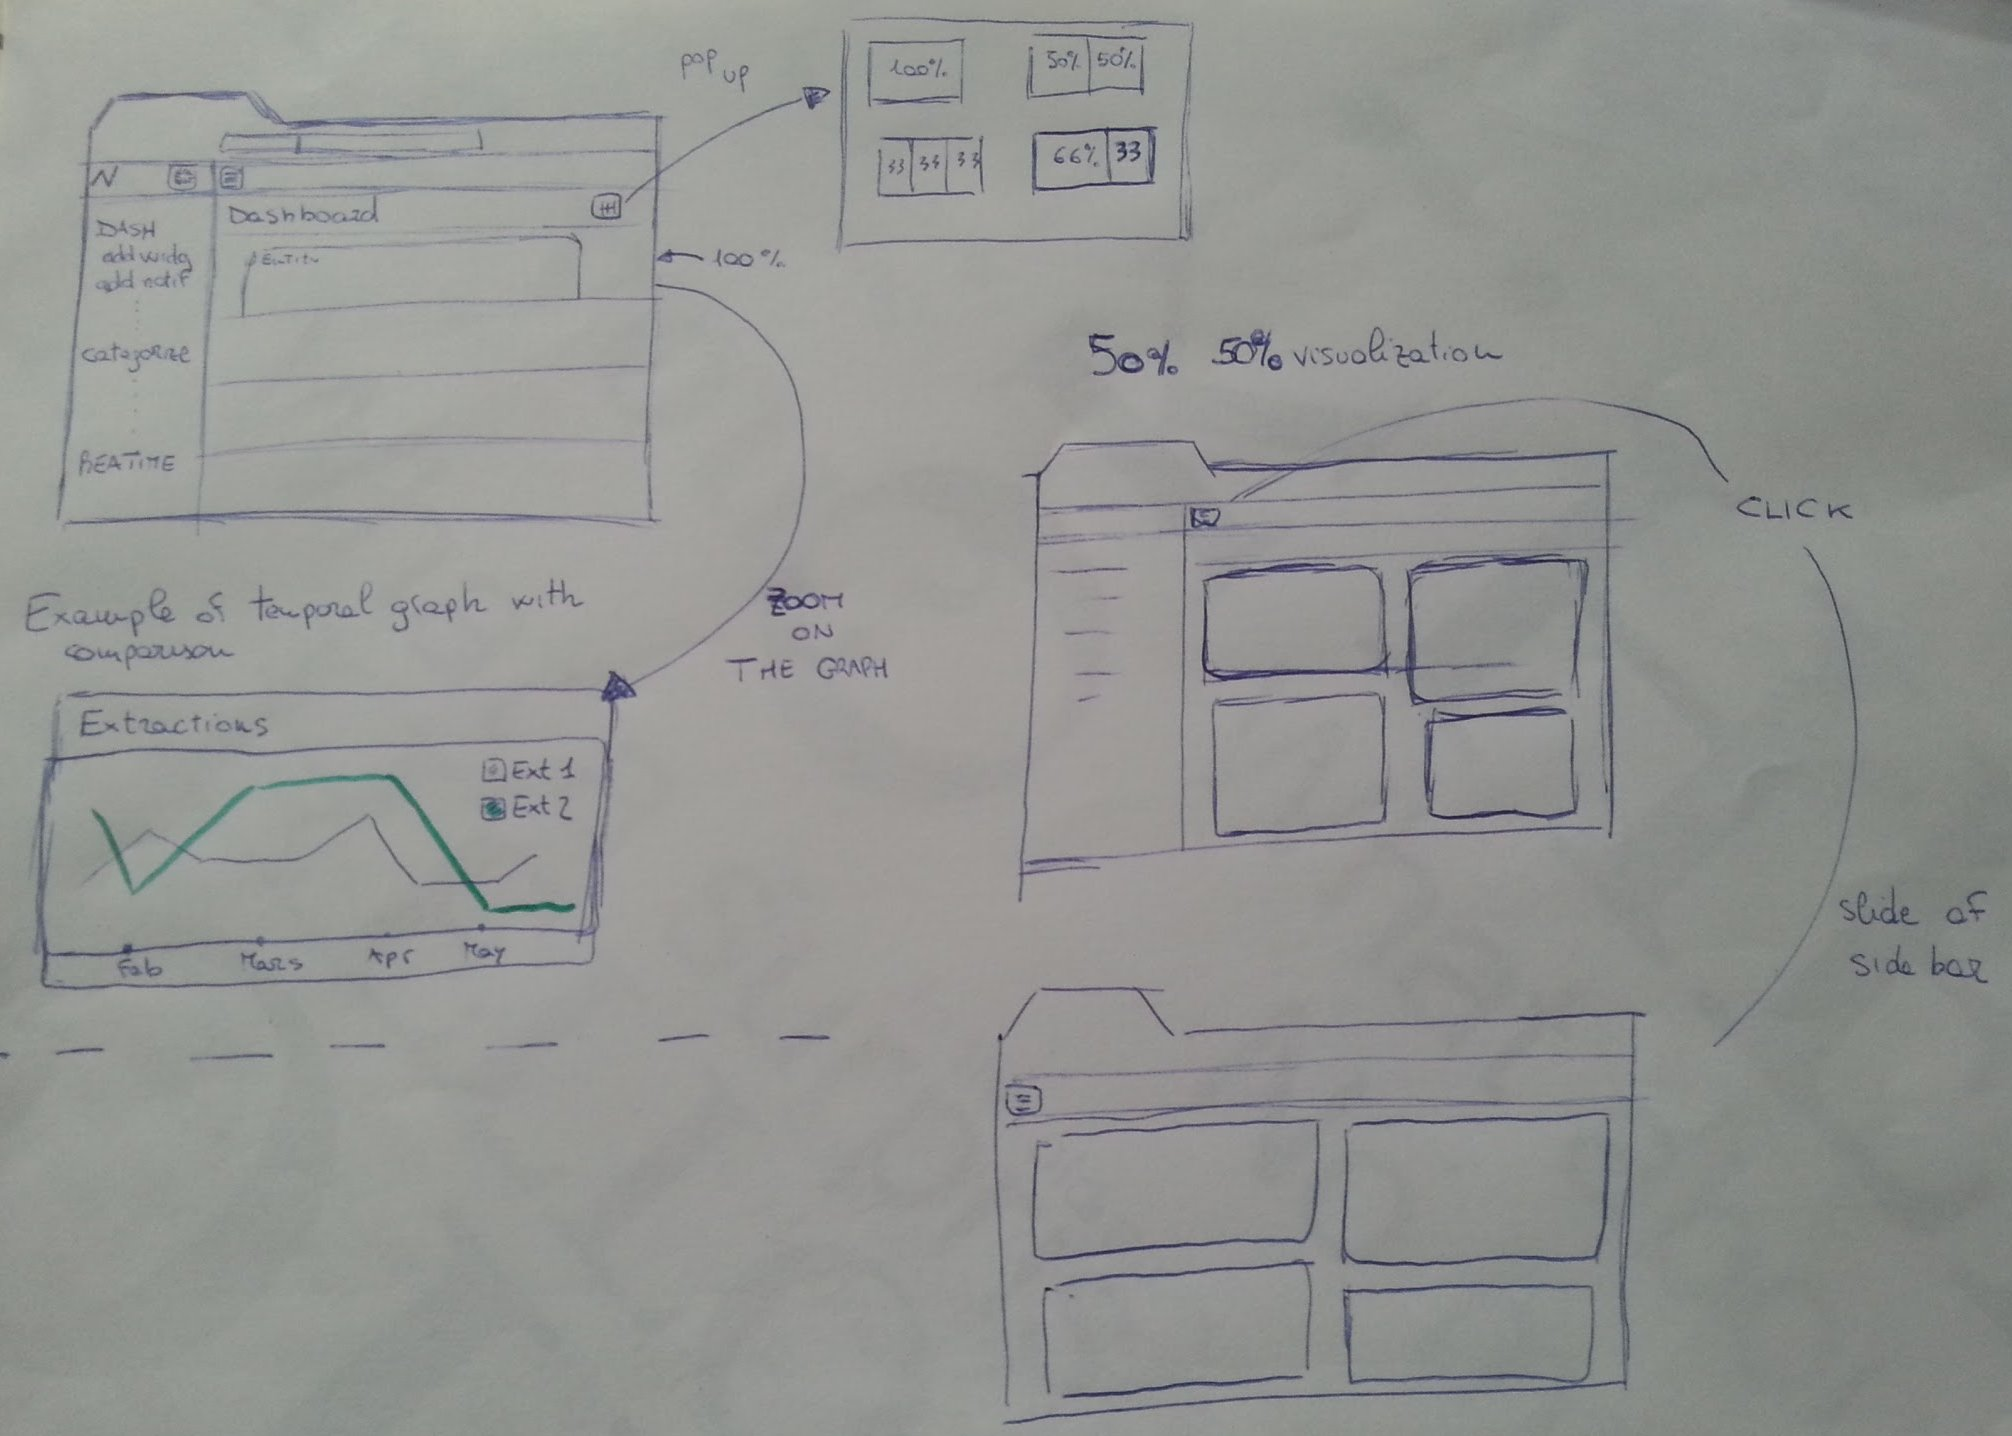
\includegraphics[width=1\textwidth]{pics/UISketches/desk0}
\end{figure}

\begin{figure}[H]
\floatbox[{\capbeside\thisfloatsetup{capbesideposition={left,top},capbesidewidth=4cm}}]{figure}[\FBwidth]
{\caption{This sketch represents the view of one section of the dashboard, the sidebar is visible and allow to directly navigate the dashboard. Timeline, pie, bar charts are the real content of the page}\label{fig:test}}
{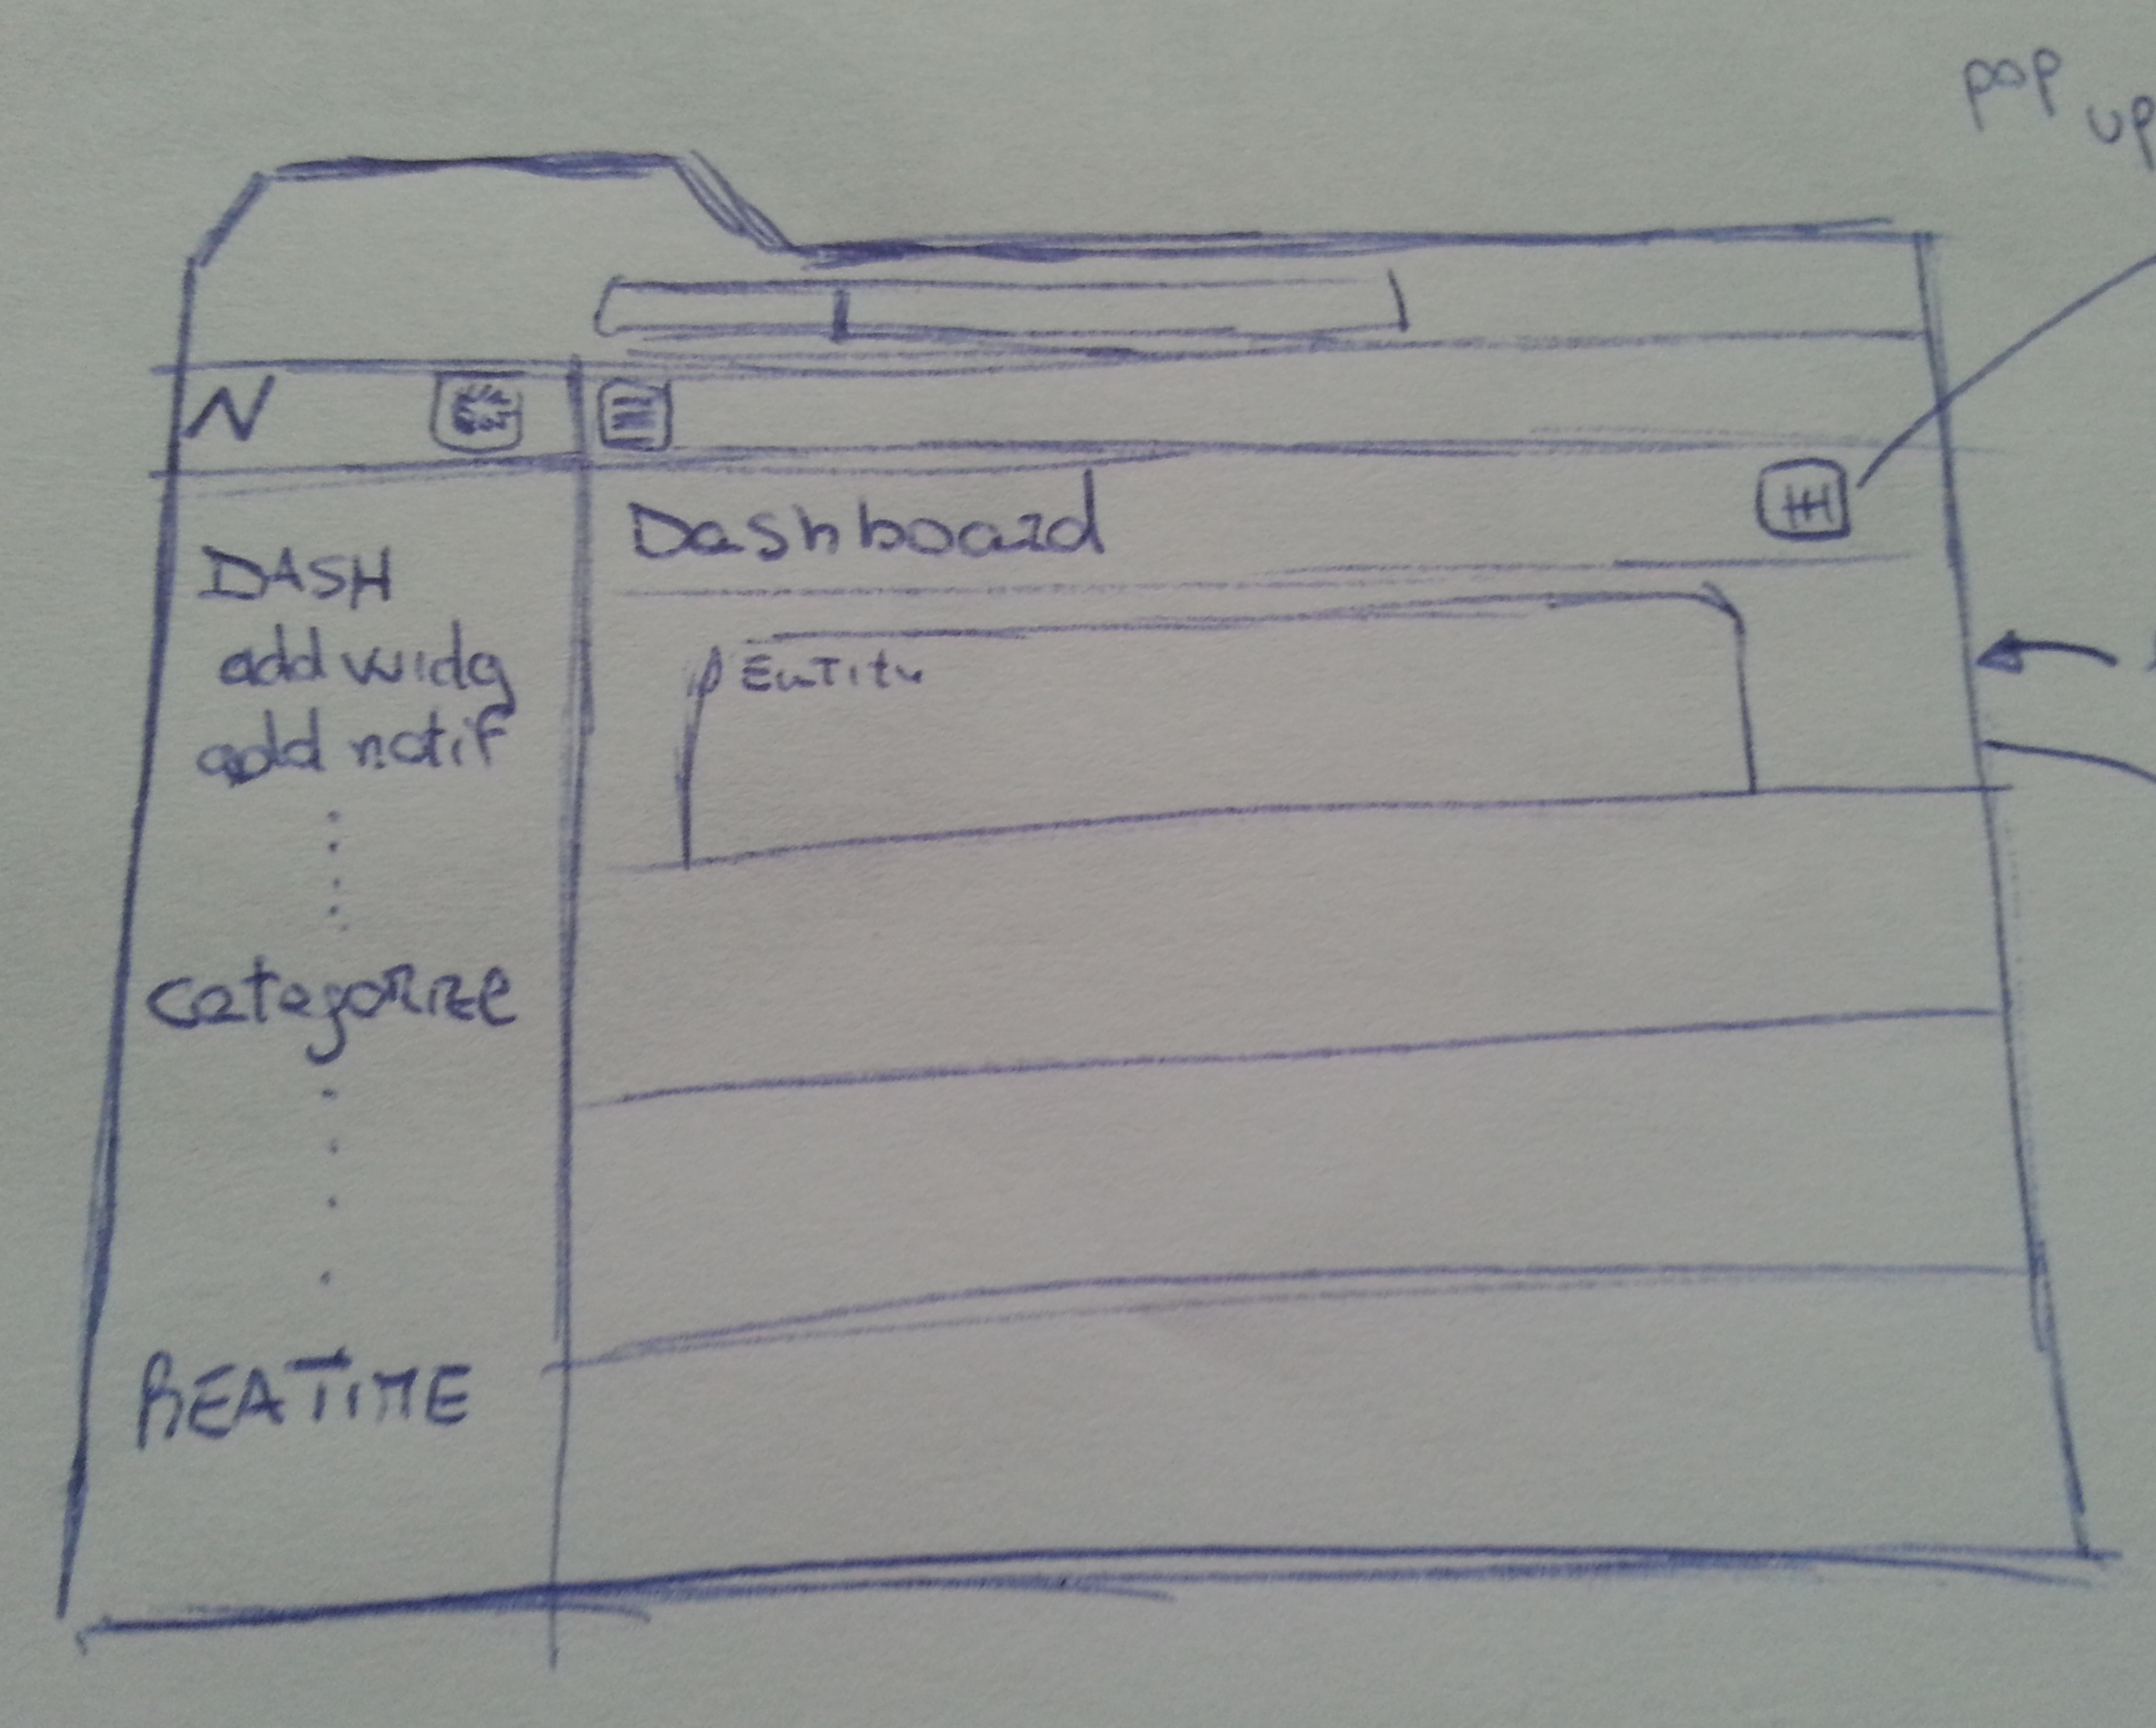
\includegraphics[width=8cm]{pics/UISketches/desk1}}
\end{figure}

\begin{figure}[H]
\floatbox[{\capbeside\thisfloatsetup{capbesideposition={right,top},capbesidewidth=4cm}}]{figure}[\FBwidth]
{\caption{From this panel, directly accessible to each section of the dashboard, the user could choose the most suitable layout, choosing between: 100, 50-50, 33-33-33, 33-66. This different configurations allow to have data differently organized in the page. }\label{fig:test}}
{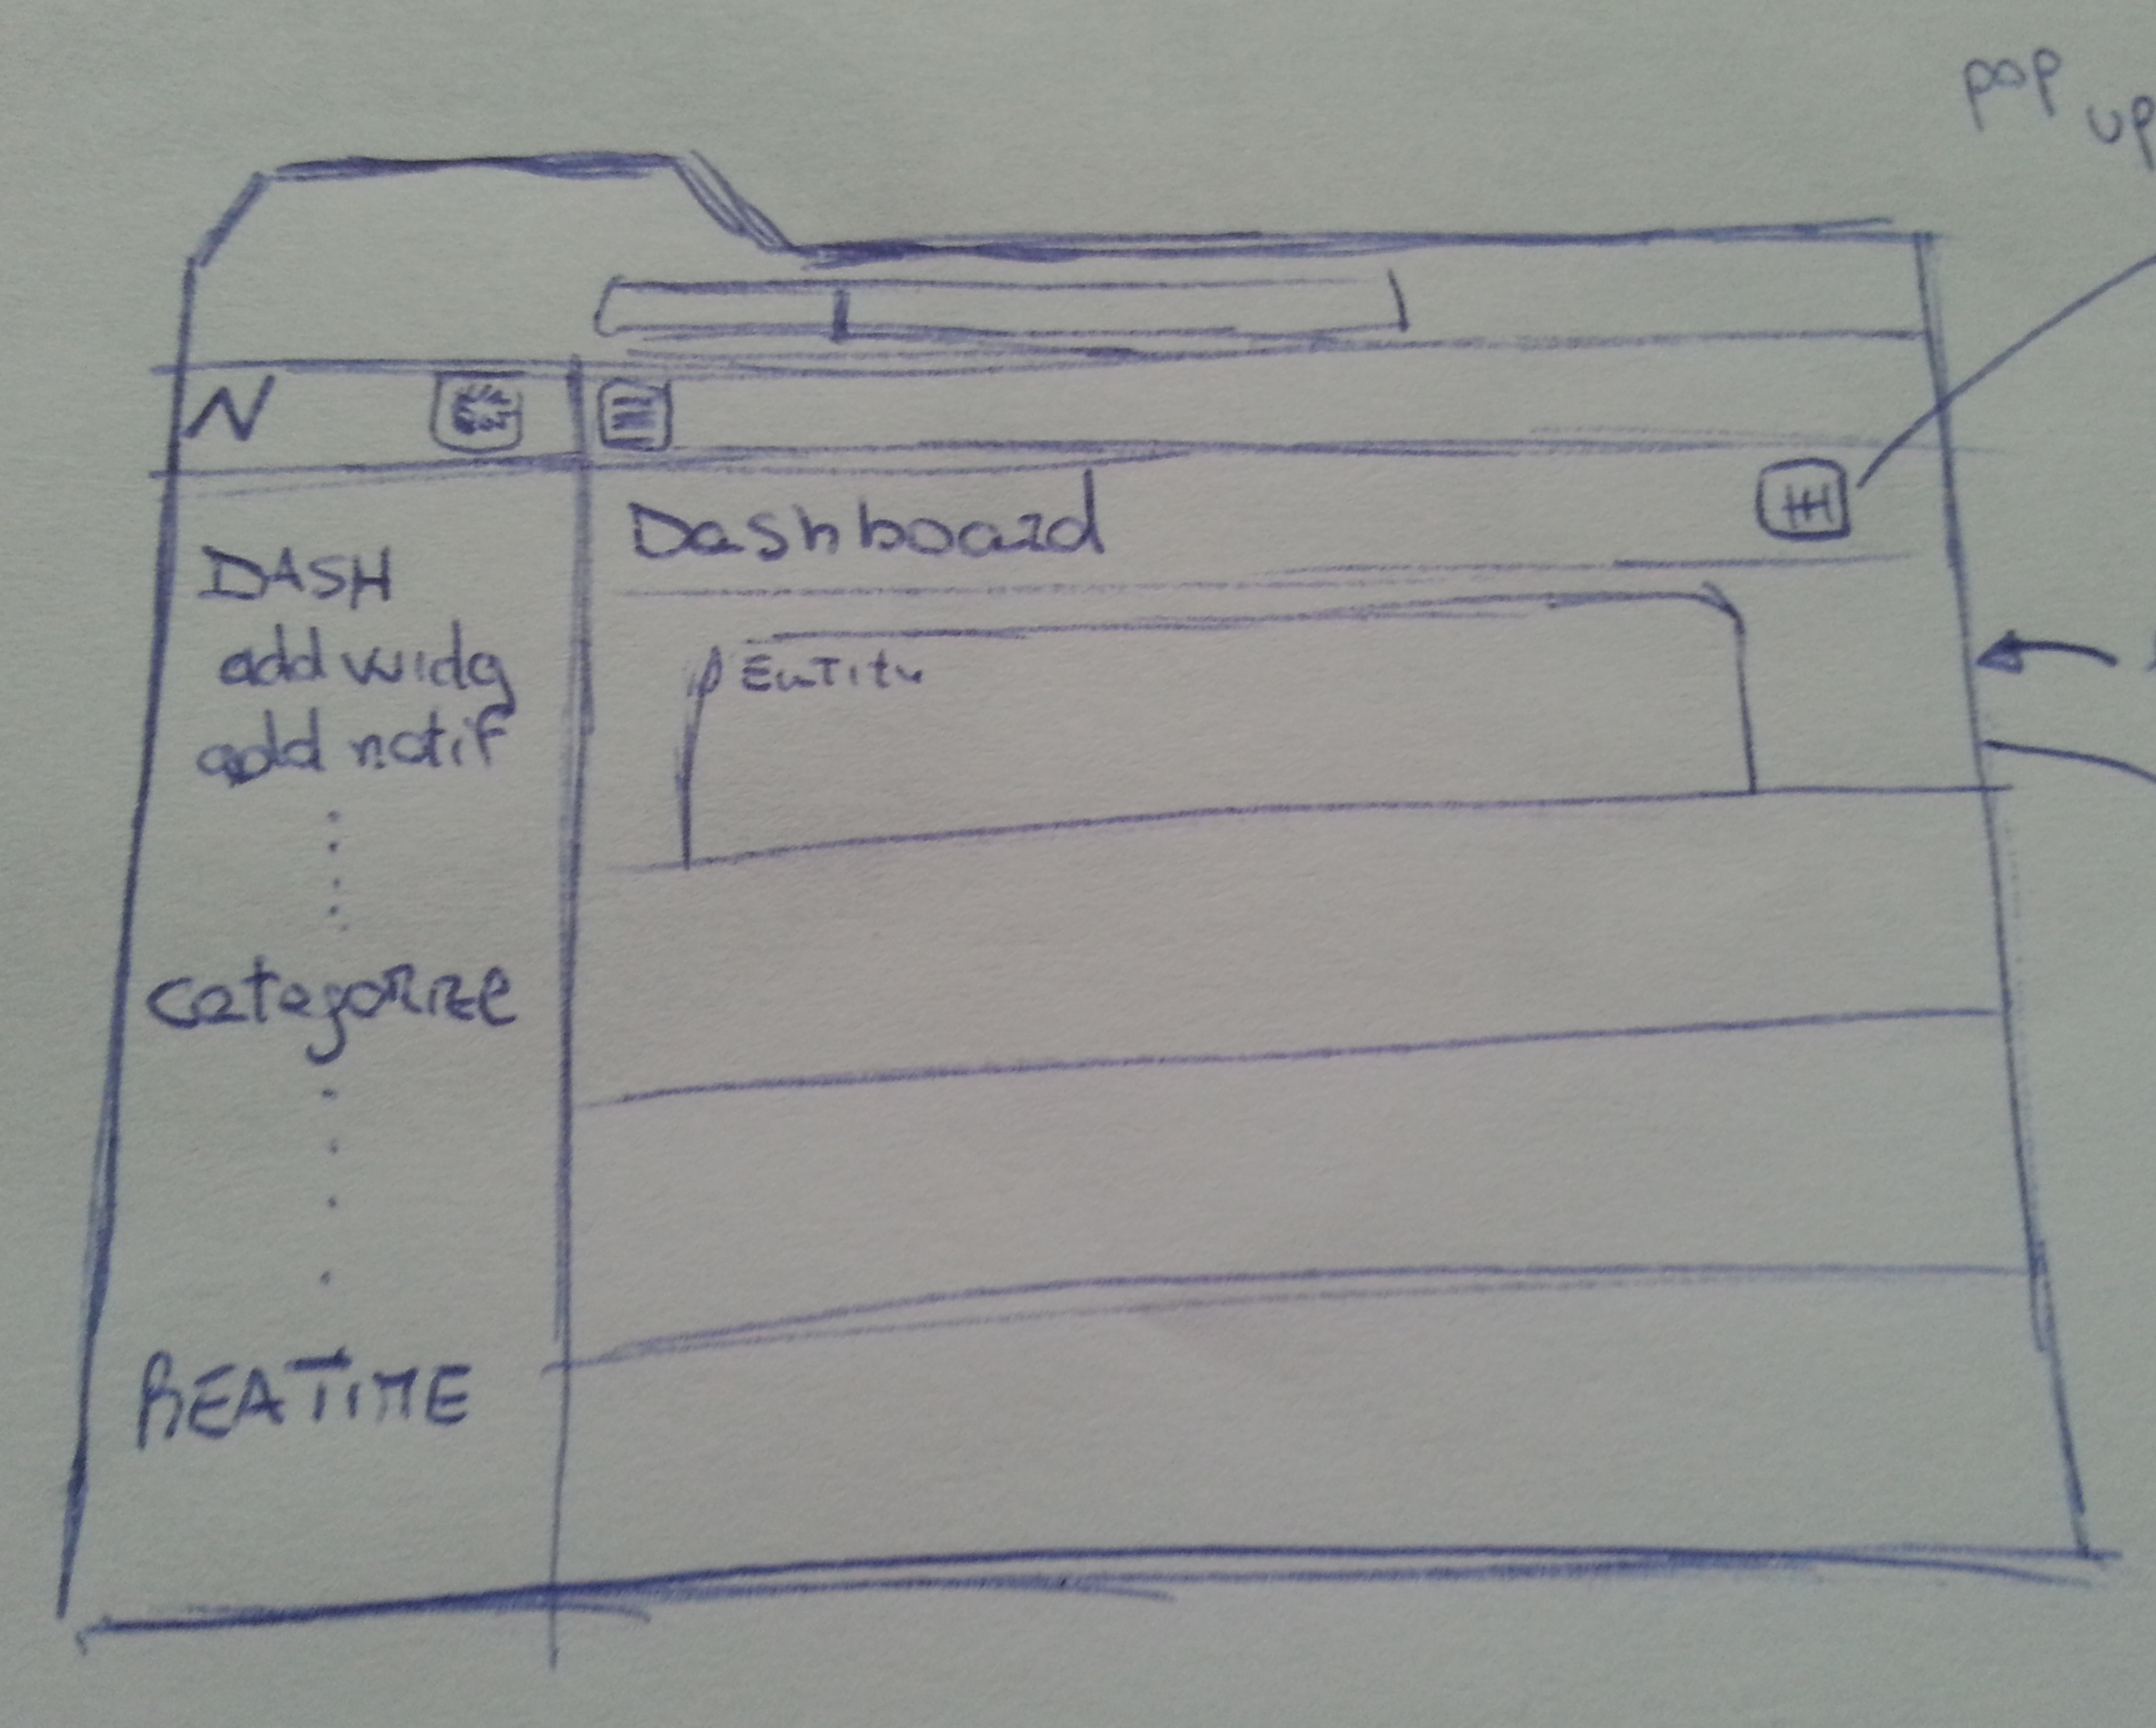
\includegraphics[width=8cm]{pics/UISketches/desk1}}
\end{figure}


\begin{figure}[H]
\floatbox[{\capbeside\thisfloatsetup{capbesideposition={left,top},capbesidewidth=4cm}}]{figure}[\FBwidth]
{\caption{This is an example of 50-50 layout making the data visualization more compact and allowing users to have the focus on more charts than the 100\% one.}\label{fig:test}}
{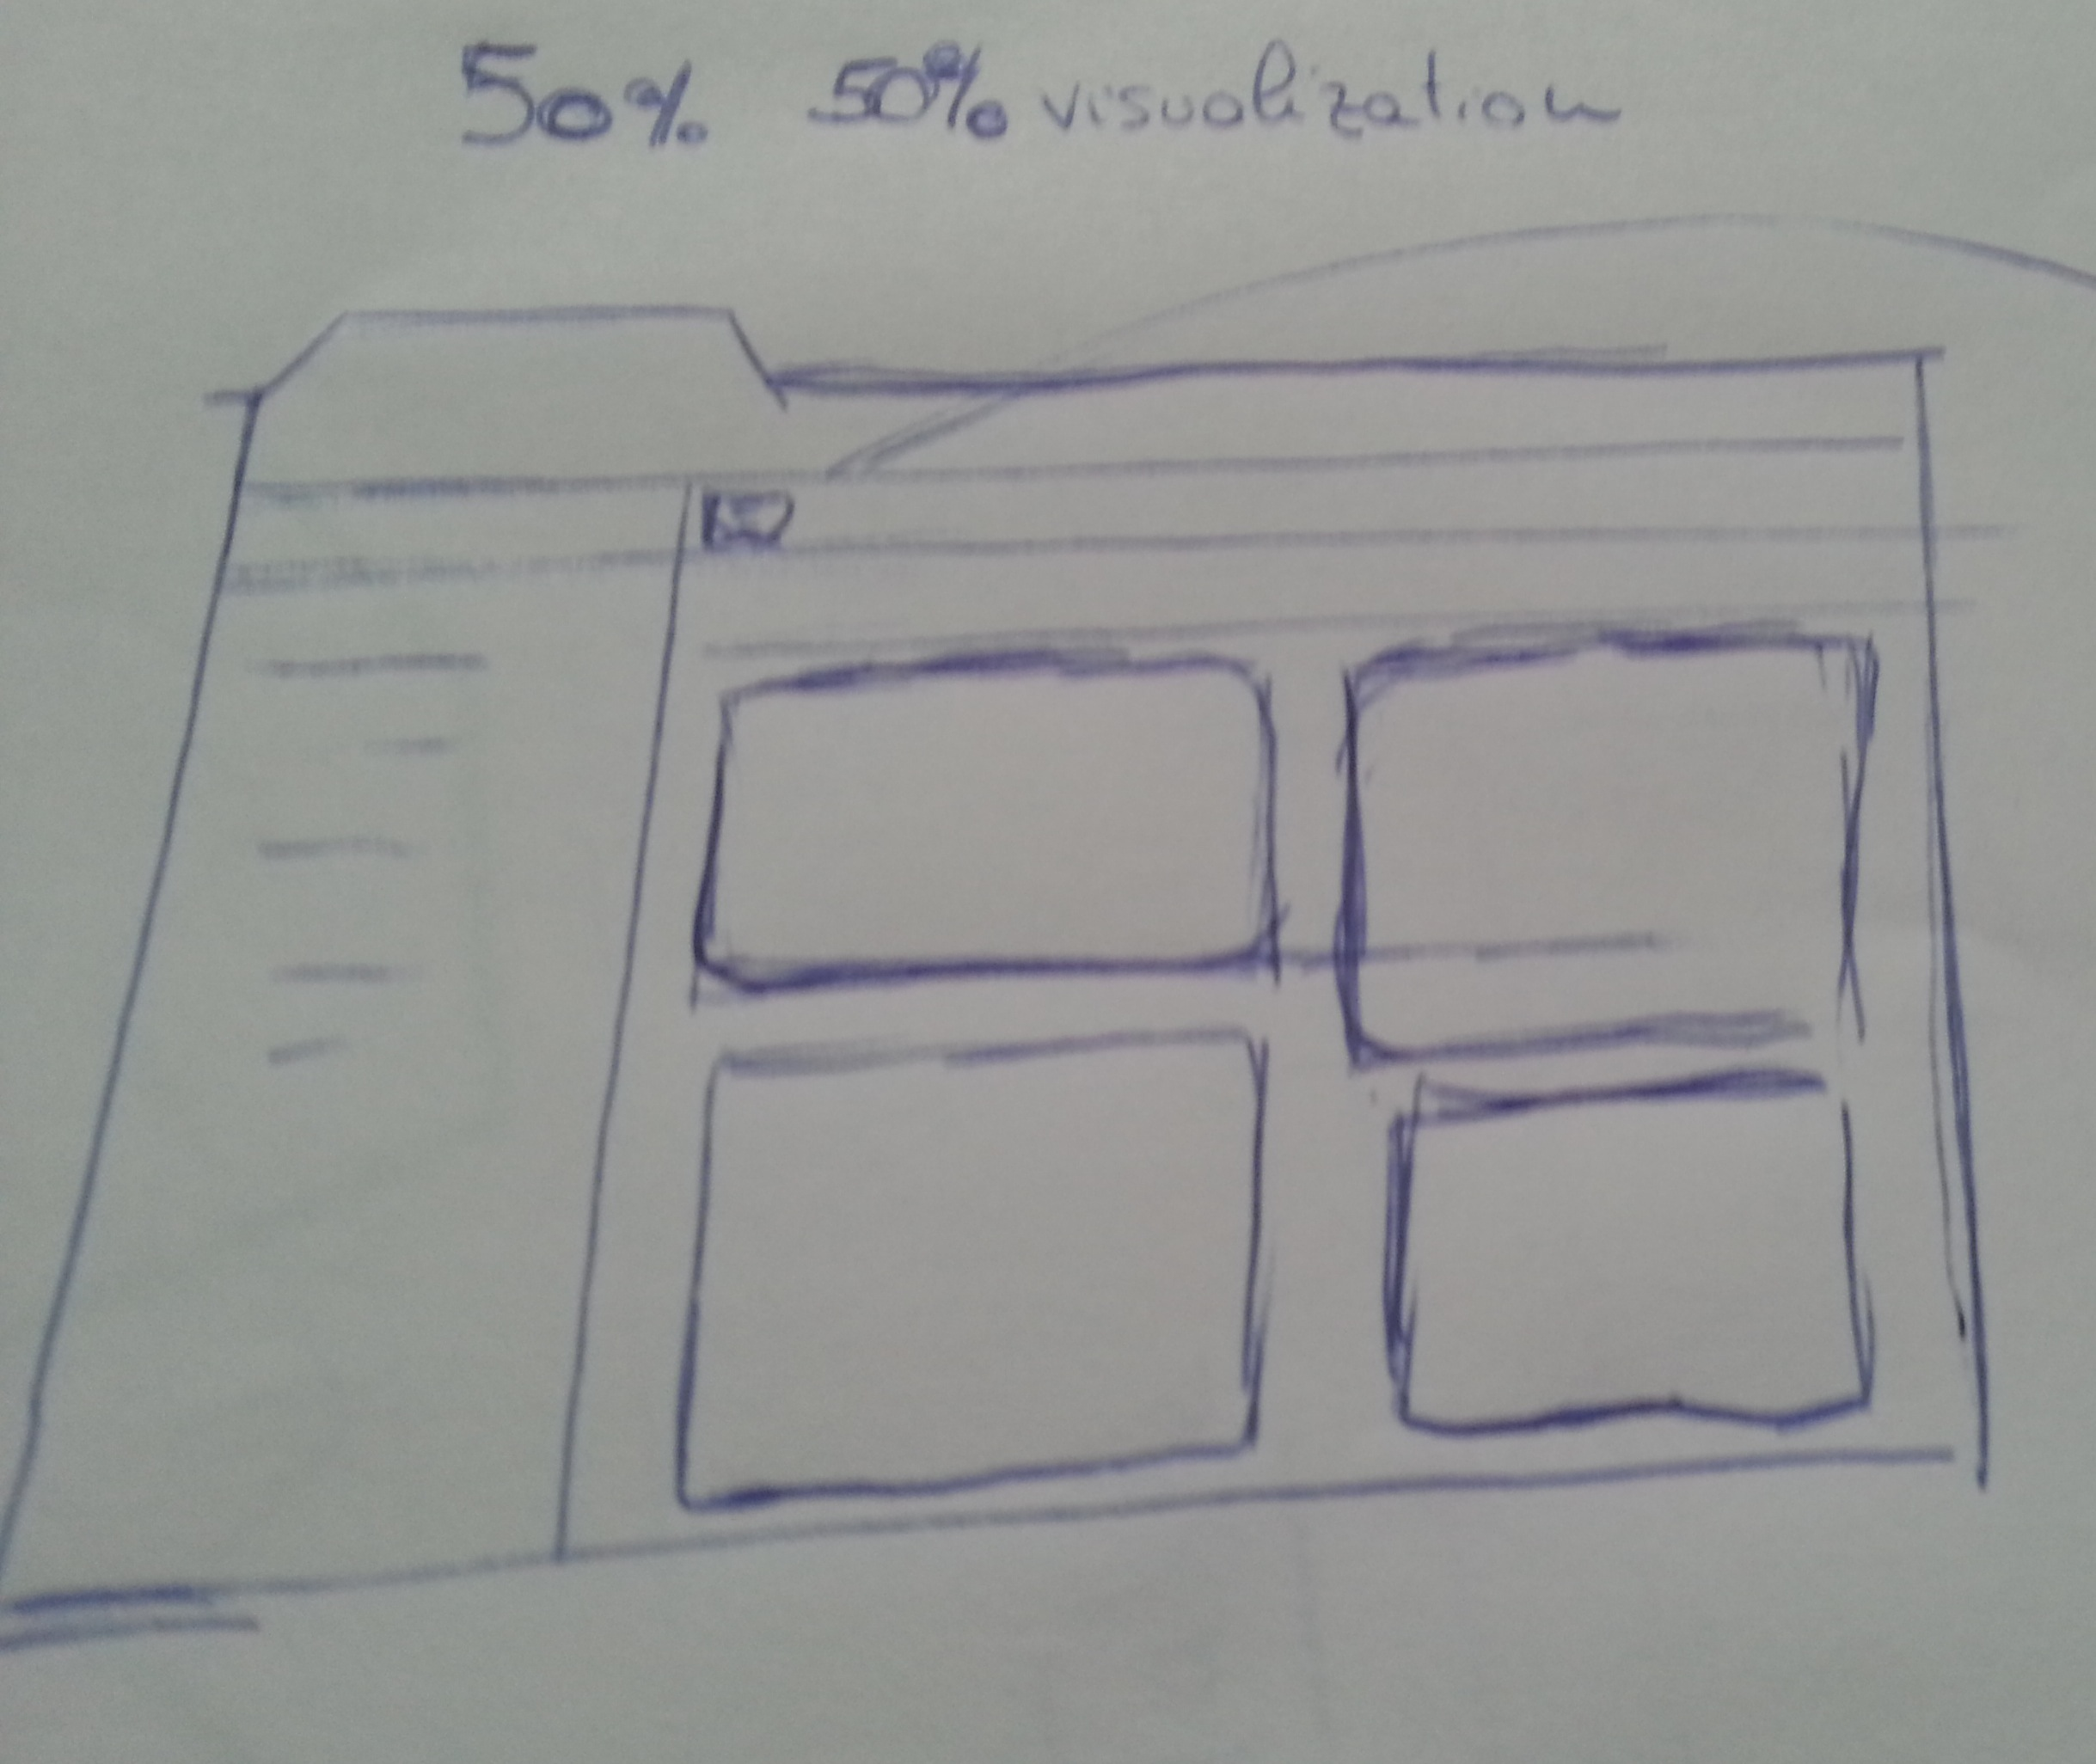
\includegraphics[width=8cm]{pics/UISketches/desk3}}
\end{figure}

\begin{figure}[H]
\floatbox[{\capbeside\thisfloatsetup{capbesideposition={right,top},capbesidewidth=4cm}}]{figure}[\FBwidth]
{\caption{This is an example of 50-50 layout in Full Screen Mode. This visualization allows to fully exploit the size of the screen: the user can focus on data without any distraction}\label{fig:test}}
{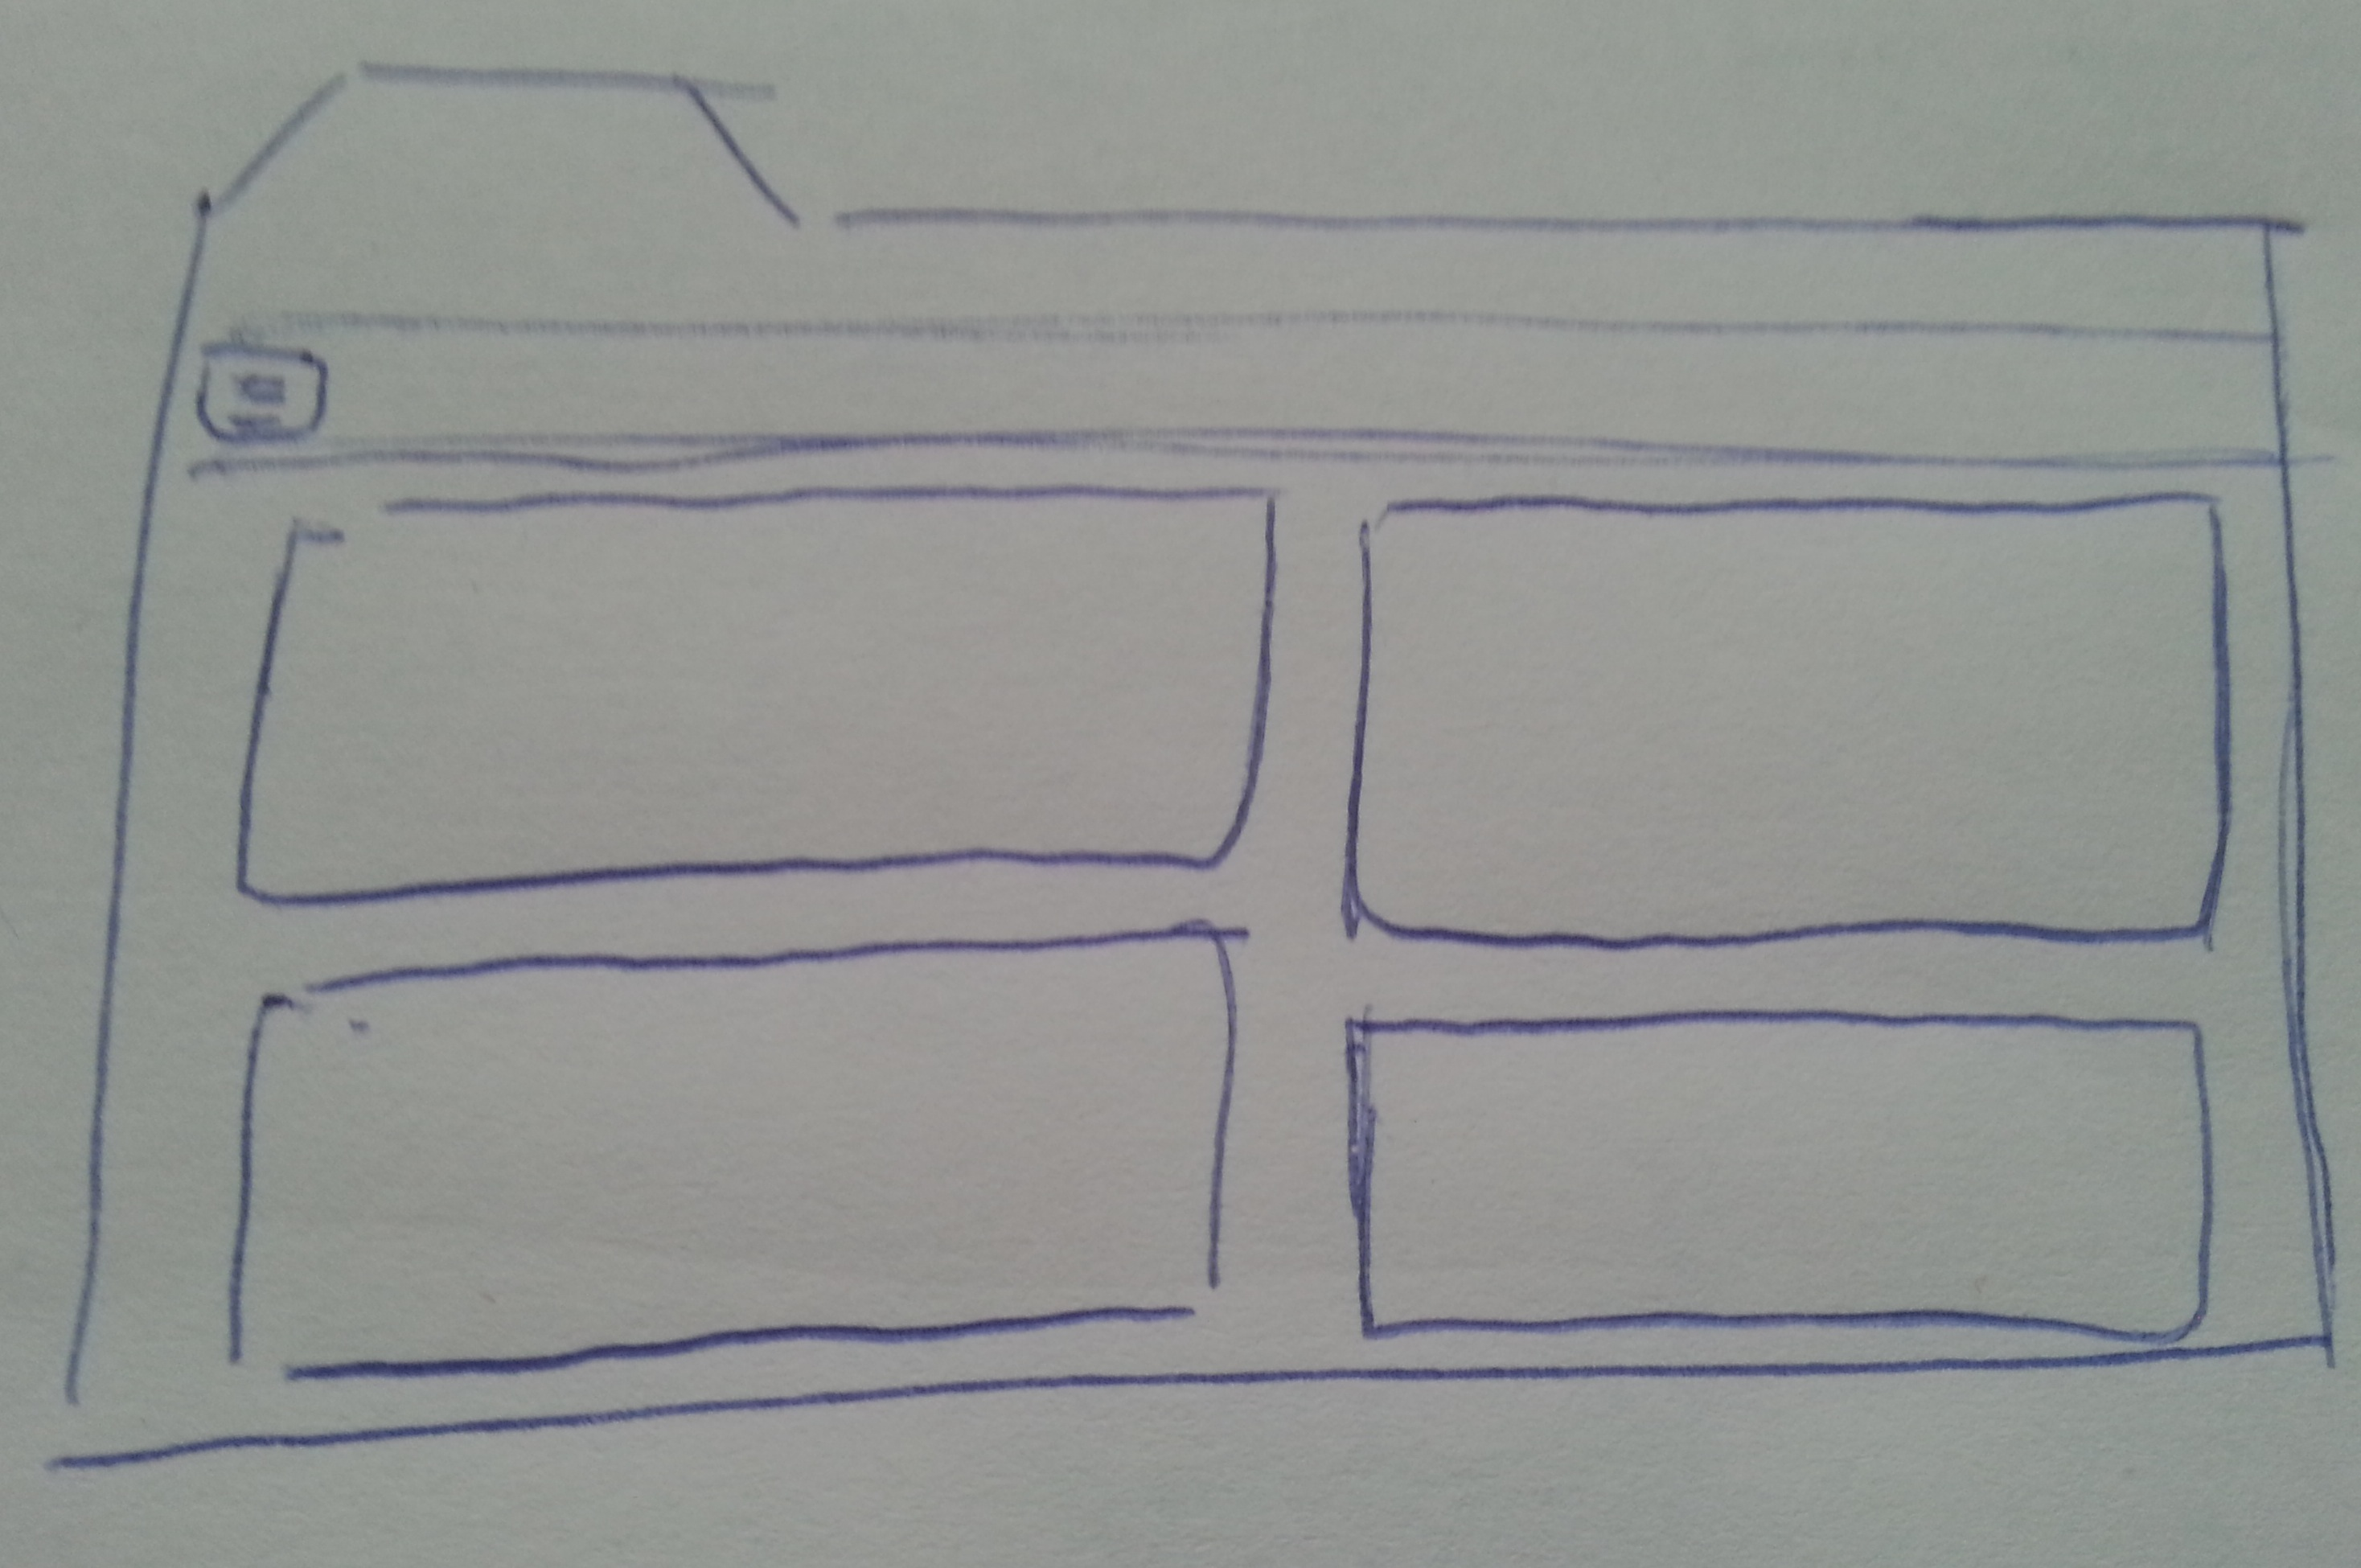
\includegraphics[width=8cm]{pics/UISketches/desk4}}
\end{figure}


\subsection{ Charts }
A dashboard needs to tell a story with data: charts and 
tables are the means to highlight the right information and make them easy to read. It's critically important to choose the right chart for the right data and to design charts visualization following this six guidelines:
\begin{itemize}
\item \textbf{Decrease data-to-ink ratio } 
\item \textbf{Maximize contrast }  Maximize the contrast between your data and the background
\item \textbf{Readable Labels } 
\item \textbf{Avoid smoothing and 3D }  Maximize the contrast between your data and the background
\item \textbf{Sort for comprehension }
\item \textbf{Use color variants }  
\end{itemize}
Starting from this principles and thinking on the type of data to display we came up with the following sketches.

\begin{figure}[H]
\floatbox[{\capbeside\thisfloatsetup{capbesideposition={right,top},capbesidewidth=4cm}}]{figure}[\FBwidth]
{\caption{This is how the graph panel should appear on the page: a top bar with the chart title(and possible icons for interaction), the graph itself and a legend}\label{fig:test}}
{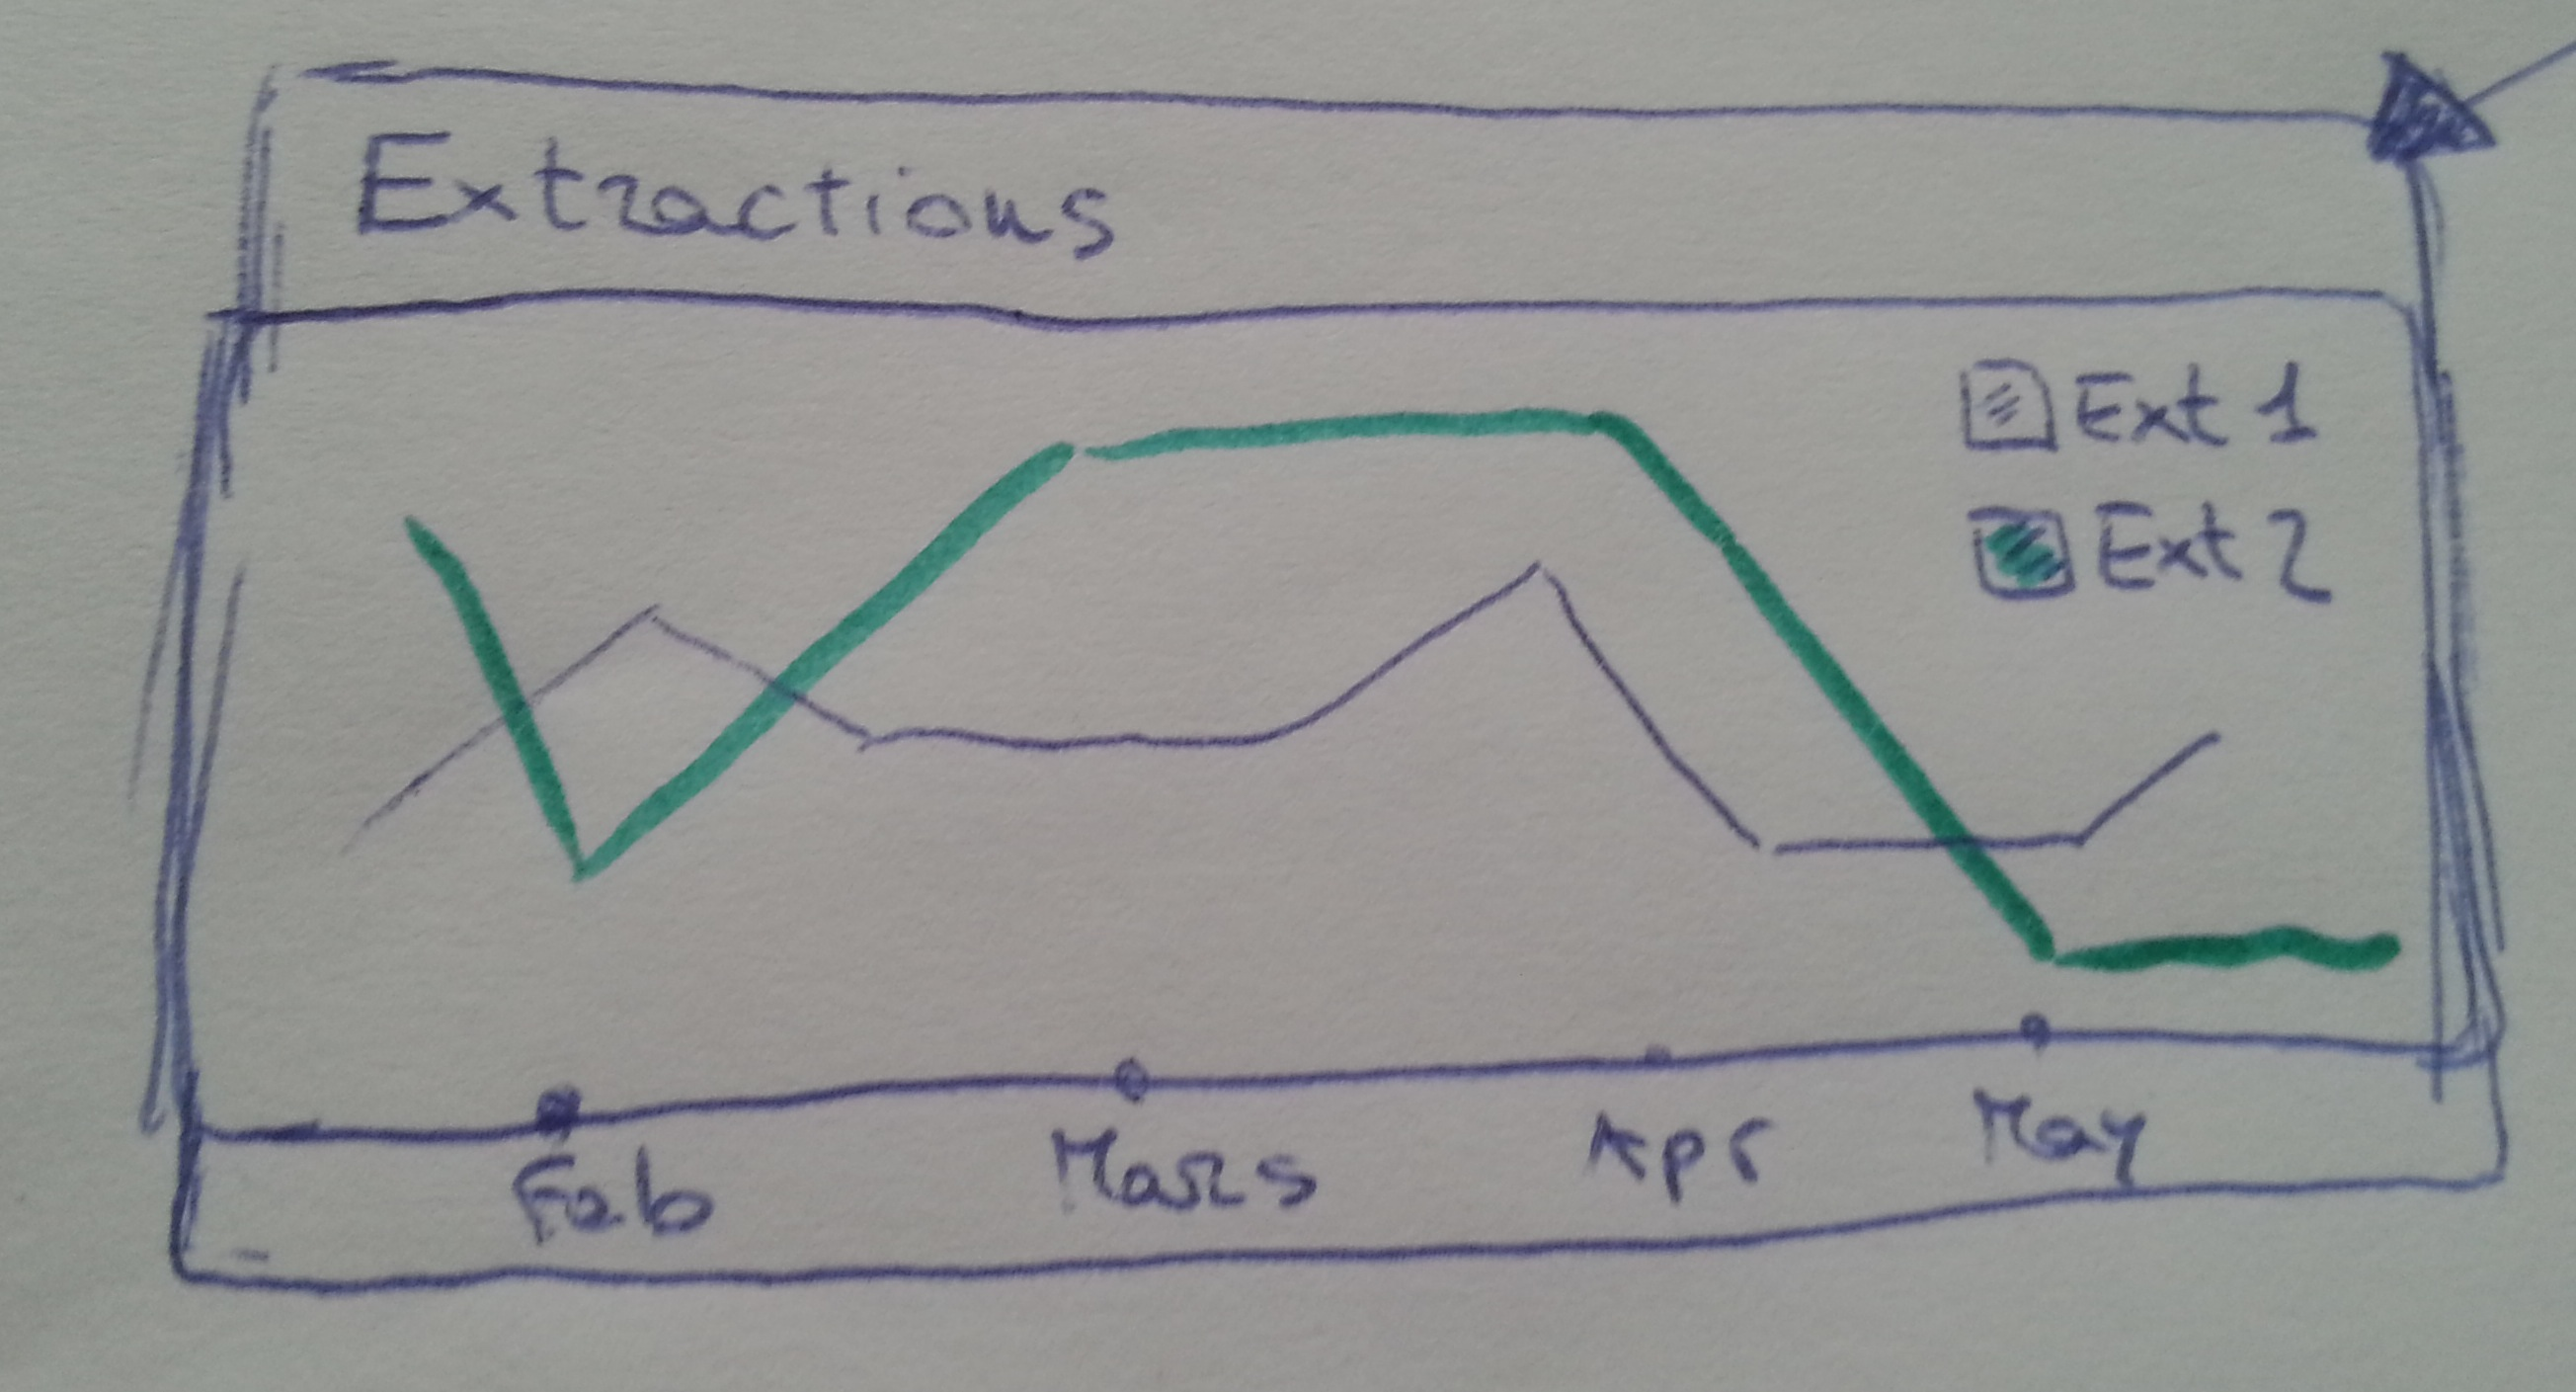
\includegraphics[width=10cm]{pics/UISketches/chart0}}
\end{figure}


\begin{figure}[H]
\floatbox[{\capbeside\thisfloatsetup{capbesideposition={right,top},capbesidewidth=4cm}}]{figure}[\FBwidth]
{\caption{Sketches of all possible type of chart for the visualization of the NERD dashboard data.}\label{fig:test}}
{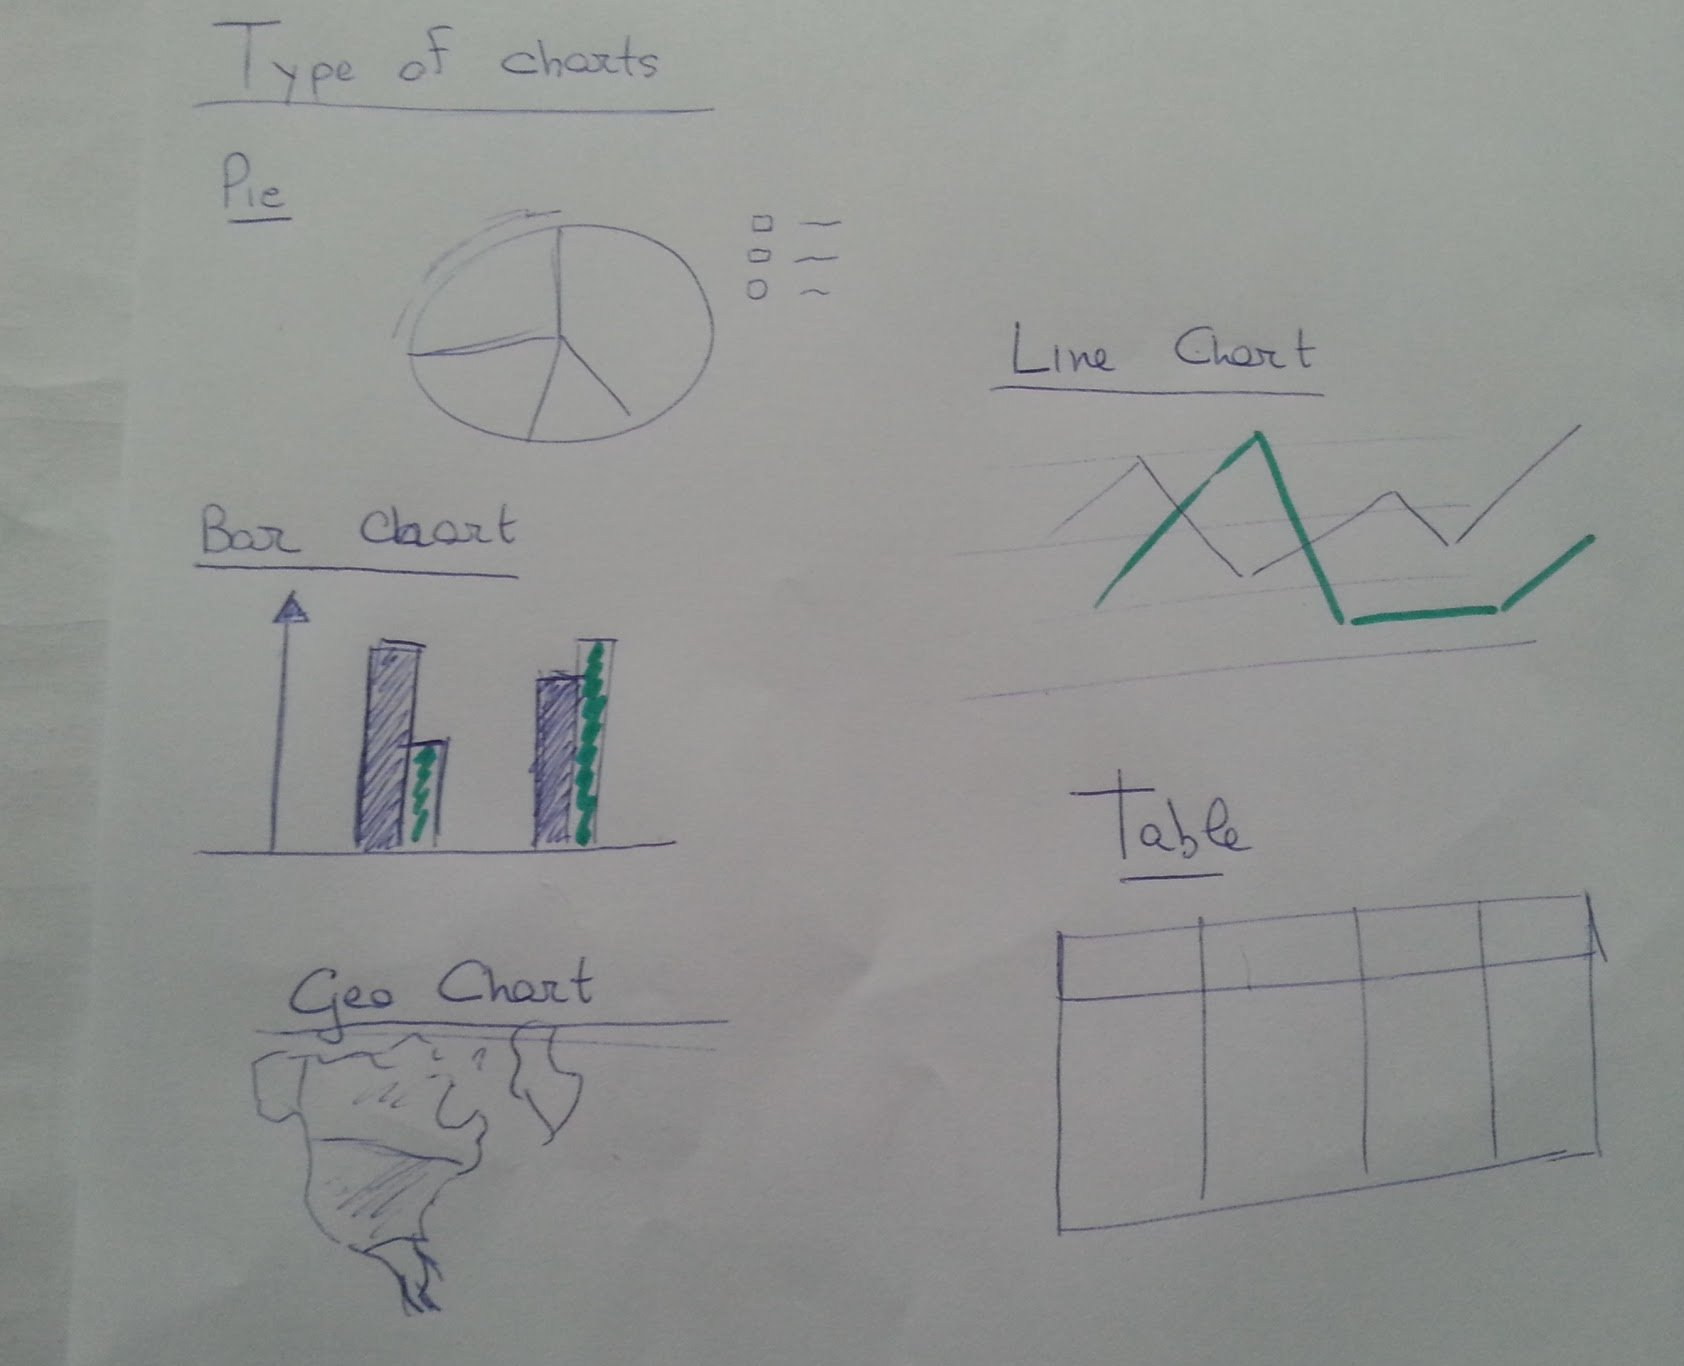
\includegraphics[width=10cm]{pics/UISketches/chart1}}
\end{figure}

\section{AngularJs}
AngularJS is a MVC framework that defines numerous concepts to properly organize a web application. It also encapsulates the behavior of your application in controllers which are instantiated thanks to dependency injection. Thanks to the use of dependency injection, AngularJS helps you structure and test your Javascript code very easily. Moreover utility code can easily be factorized into services that can be injected in your controllers.\newline
According to Wikipedia the goal of Angular is to augment browser-based applications with model-view-controller (MVC) capability but this isn't enough to fairly describe the potentialities of this Frameworks.
The capabilities of this framework could be summarized with the ``3D of Angular'': Directives, Data Binding and Dependency Injection.\newline
\textbf{Directives} are one of the most innovative feature of Angular and what makes Angular different from all the other client-side MVC frameworks. Directives ``are a way to teach HTML new tricks'' and allow the developer to create new HTML elements for your own needs: Angular takes care to match and execute during the DOM compilation.
The power of directive relies on allowing the developer to create reusable and flexible widgets which can be used anywhere in your application and even outside. Moreover the HTML become more readable and concise.
\newline
\begin{quotation}
  Then we have Data-binding that according to the AngularJs website can be defined as the automatic way of updating the view whenever the model changes, as well as updating the model whenever the view changes. This is awesome because it eliminates DOM manipulation from the list of things you have to worry about.
\end{quotation}

Finally we have Dependency injection is a design pattern that allows to make test driven development easier. With dependency injection it's easy to transparently load mocked objects in tests, which means test the modules separately and independently from the system logic.

 \section{Setting up the Development Workflow}
 Nerd Dashboard has been developed using a few cool tools that make the developer life easier. 

One of the first tool to be aware of is Grunt which is a Javascript Task Runner. Grunt allows to automate repetitive tasks like minification, compilation, unit testing, linting, etc, the easier your job becomes.\newline
Another tool intensively exploited is Compass, a CSS Authoring Framework built on Sass ( an extension of CSS3 which adds nested rules, variables, mixins, selector inheritance).
Last but not the least is Yeoman 1.0: a collection of tools and best practices working in harmony to make developing for the web even better. Actually Yeoman could be considered a workflow that comprise three tools : yo (the scaffolding tool), grunt (the build tool) and bower (for package management). As we can see we already talked about Grunt, so the last tools we have to talk about are yo and bower.

The first allows to scaffolds out a new application, writing your Grunt configuration and pulling in relevant Grunt tasks that you might need for your build ( in our case allowed to first scaffold an AngularJS application, write the Gruntfile and moreover allows with a simple instruction to scaffold new view, controllers, services for the web application). Bower is another great tool and allows to easily face the front-end package management: it is basically a package manager for the web.

\section{Building the client}
We firstly create a responsive layout for the web App that fairly followed the sketches we've done in the first design phase, creating a layout that echoes the iOs  apps for iPad.
The layout responds in different ways in desktops, tablets and smartphone in order to guarantee the best UX on each device.
We strongly used Twitter Bootstrap, but in order to achieve our goals and the responsiveness of the layout we fully customize the CSS.
For the animations of the fixed side bar I used the new CSS3 transitions and transform attributes.
We made also studies on performances on mobile devices. Initially the animation wasn't fluid, but we propose to use transform3d CSS3 attributes which makes the animation hardware accelerated.
\begin{figure}[H]
  \caption{Template on desktop screen.}
  \centering
    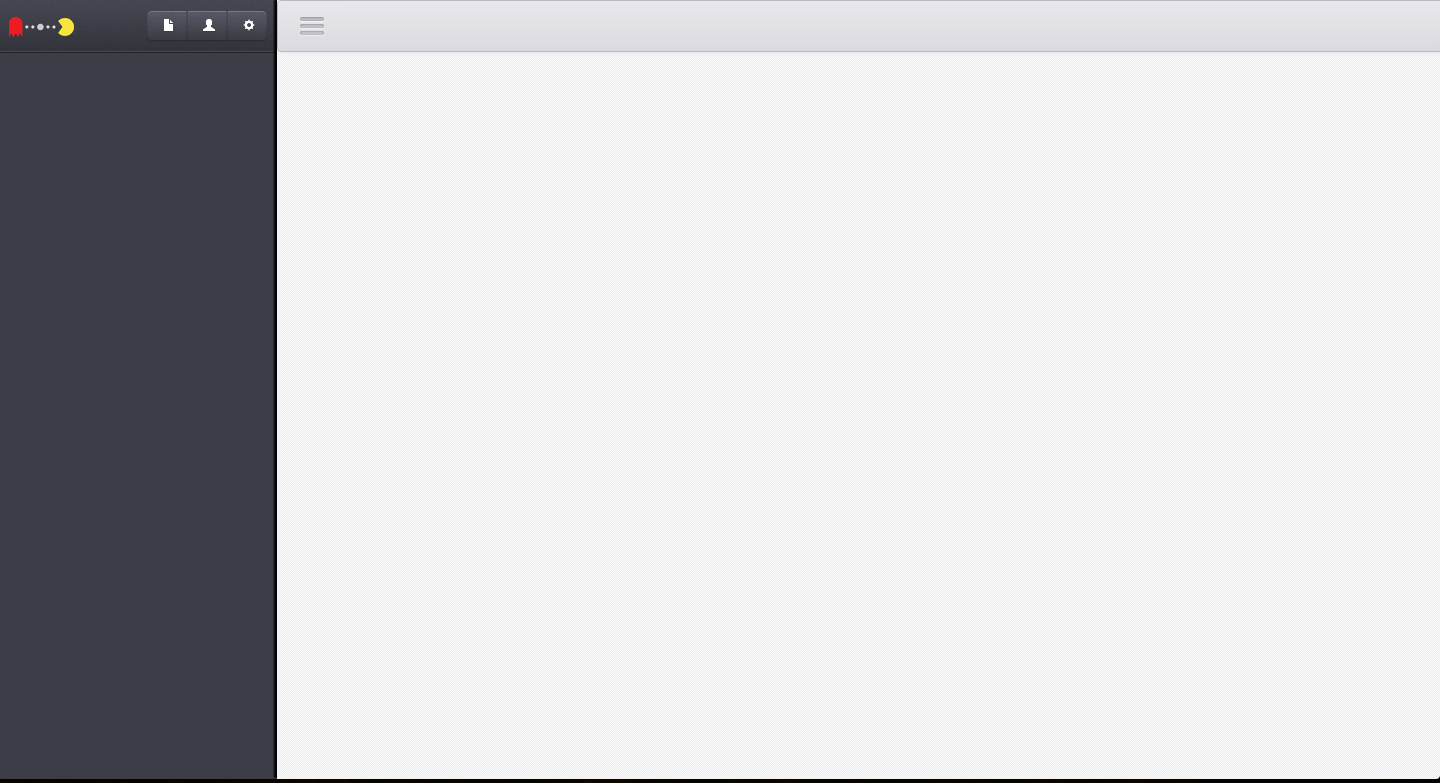
\includegraphics[width=0.9\textwidth]{pics/proto/desktopEmpty}
\end{figure}\begin{figure}[H]
  \caption{Template on tablet  and mobile screen.}
  \centering
    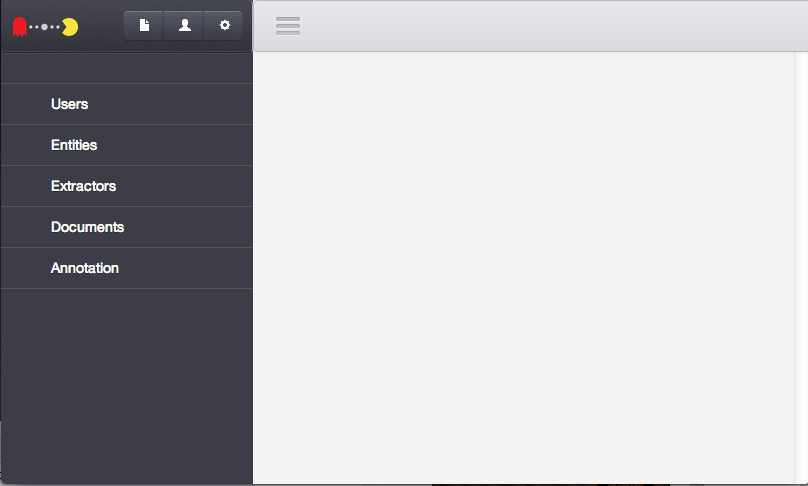
\includegraphics[width=0.5\textwidth]{pics/proto/tabletEmpty}
    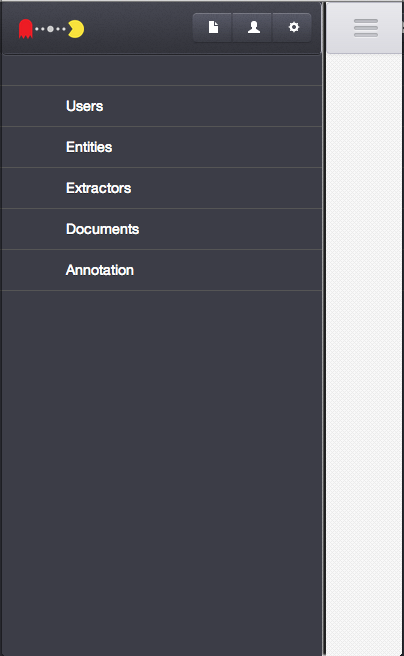
\includegraphics[width=0.3\textwidth]{pics/proto/mobileEmpty}
\end{figure}

As you can see on the pictures the sidebar is less than the 20\% on desktop screen, bigger on tablet screens and lastly on the mobile occupies the most of the page.
\section{Google Charts APIS}
NERD Dashboard first aim is to display data to the administrators therefore choose the right client interactive data visualization library is crucial to reach a good result.
After a  conscientious research through the most popular Javascript libraries for display data our choice falls on Google Charts APIs.
Google APIs exposes a lot of features from simple charts to complex hierarchical tree maps plus mechanisms to query data form external data sources.
Create simple charts is straightforward, simple as loading the module you need, passing a data Object that represents the information you want to display to a static method that takes care to draw your chart.
Unfortunately, this wasn't enough for our goal therefore we customized and wrapped the APIs to allow responsive features and in particular to create a navigation and easy aggregation of data. For example in the timeline chart, we can navigate data by time, aggregate it by day, week, month and year, this feature was added to the existing APIs 

\section{Directives}
The great work behind the client development resides on the creation of the directives, that in our case are represented by the charts widgets.
This allows to have reusable chart flexible enough to work in different context and with different data.
We code four main directives: timeline, pie chart, geocharts and modals.
\subsection{Timeline - pieChart - geocharts Directives} % (fold)
This directive is the one that takes care to make usage of the Charts APIs, to handle data coming form the angular controller.
Mainly it `'watches`' for data passed by the controlled to be fully retrieved from the server, instantiates the chart objects and call the method to draw it.
However this isn't the only stuff that it has to handle; this directive also takes care to draw the navigation elements, set event handler on them, redraw the graph for different screen size, define different navigation methods depending on the user agent( the navigation on the temporal axis for the timeline directive is made with buttons for desktop application and with swipe on tablet and mobile version.
\begin{figure}[H]
  \caption{Timeline Directive}
  \centering
    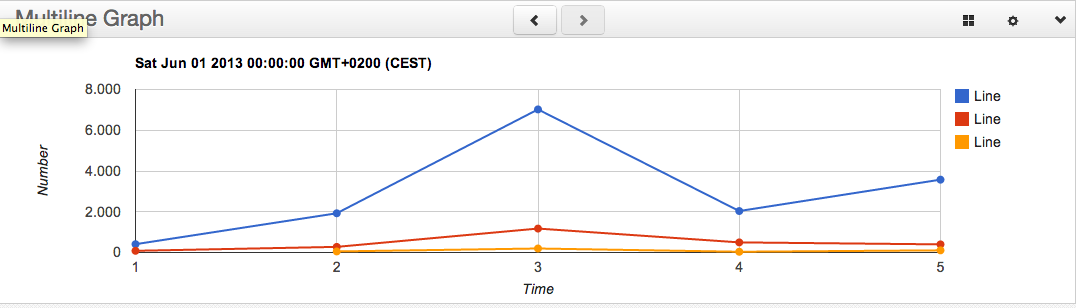
\includegraphics[width=1\textwidth]{pics/proto/timeline}
\end{figure}
\begin{figure}[H]
  \caption{Geochart and PieChart Directive.}
  \centering
    \includegraphics[width=0.489\textwidth]{pics/proto/geoChart}
    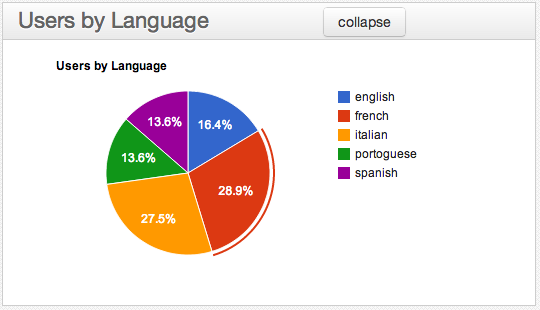
\includegraphics[width=0.489\textwidth]{pics/proto/pieChart}
\end{figure}
\subsection{Modal Directive} % (fold)
Administrator can handle the settings of his charts (add lines and define filters) through an handy modal window.
This work is made by a directive that takes care to draw the modal itself, register events handlers on the DOM elements and to delegate the effective work of calling Server APIs to retrieve data and register - retrieve filters to the right controllers. Moreover, for entities and annotations it offers a auto-complete for filters value that transparently retrieves the possible choices from the server.
\label{sub:modal_directive}
\begin{figure}[H]
  \caption{Modal Directive.}
  \centering
    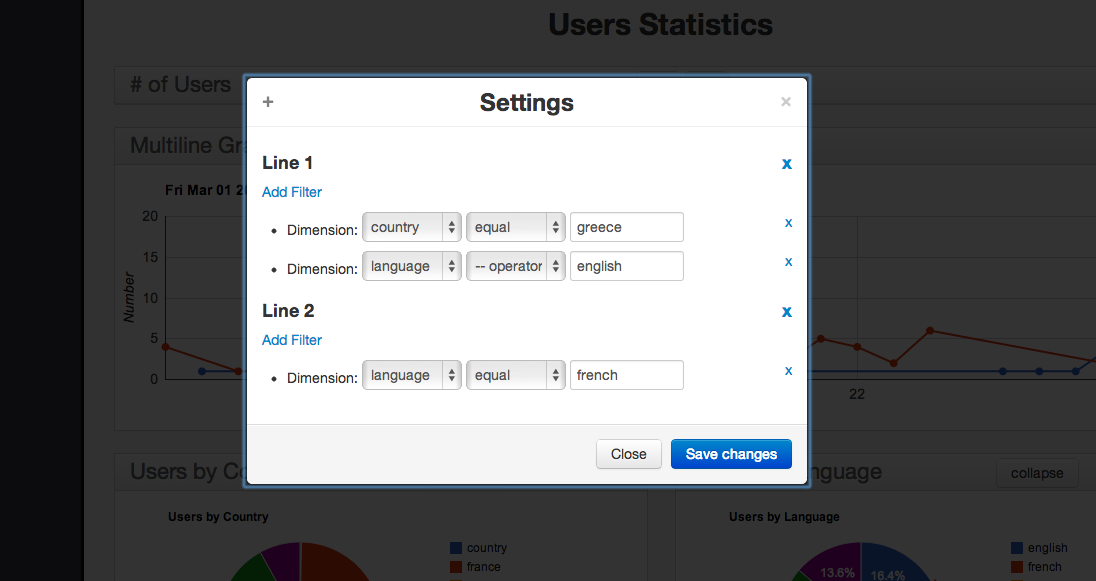
\includegraphics[width=1\textwidth]{pics/proto/modalOptions}
\end{figure}
\subsection{Services} % (fold)
\label{sub:services}
Angular exposes a nice service to handle REST APIs calls: `'\$resource''.
We decided to wrap this Angular service for our resources in order to have an easier interface from the controller to access data coming from the server.
Moreover, to build the nice navigation in the timeline graph we already talk, we had to heavily manipulate data coming from the APIs calls, in order to have data structures suitable for our timeline directive.
\begin{figure}[H]
  \caption{Screenshot of the final result on big desktop screen.}
  \centering
    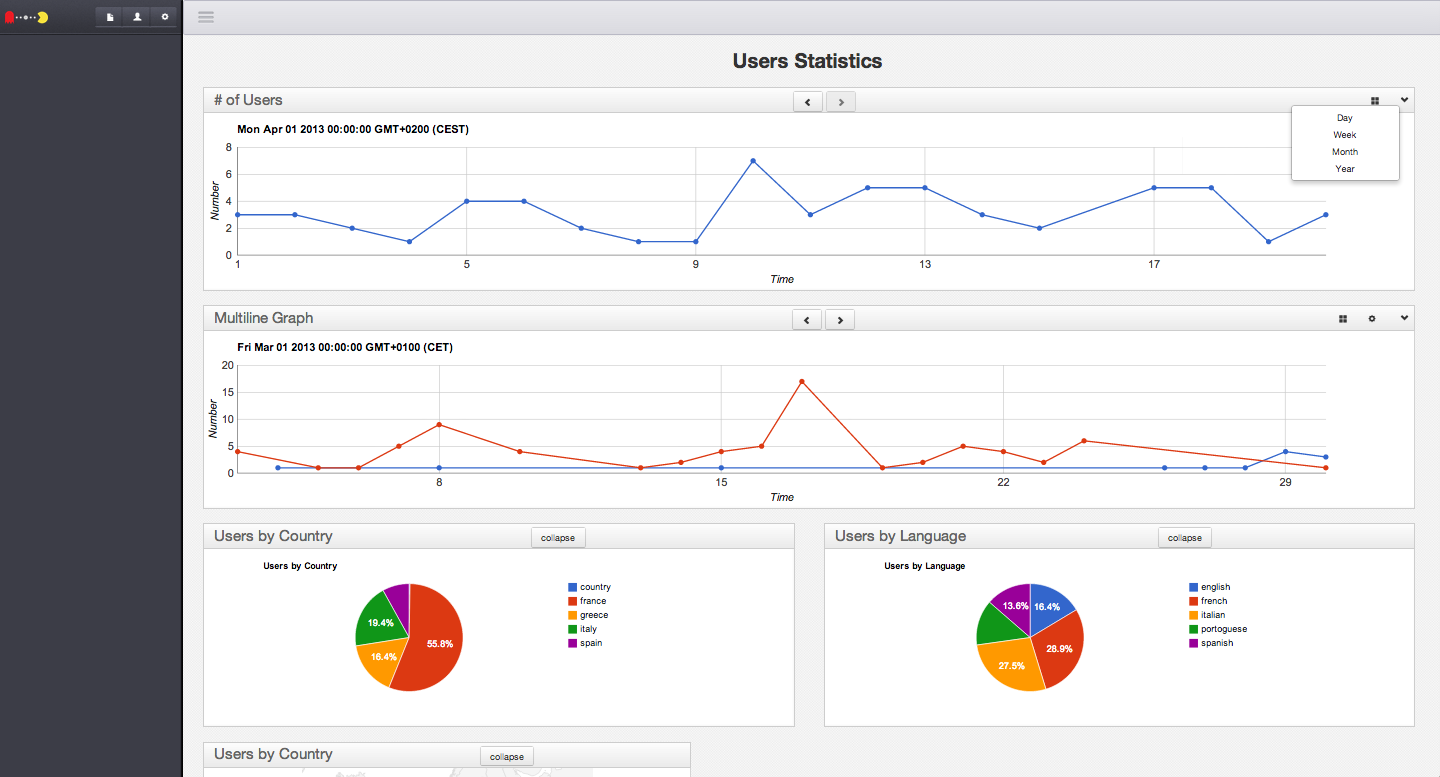
\includegraphics[width=1\textwidth]{pics/proto/fullDesktop}
\end{figure}
\begin{figure}[H]
  \caption{Screenshot of the final result on big desktop screen}
  \centering
    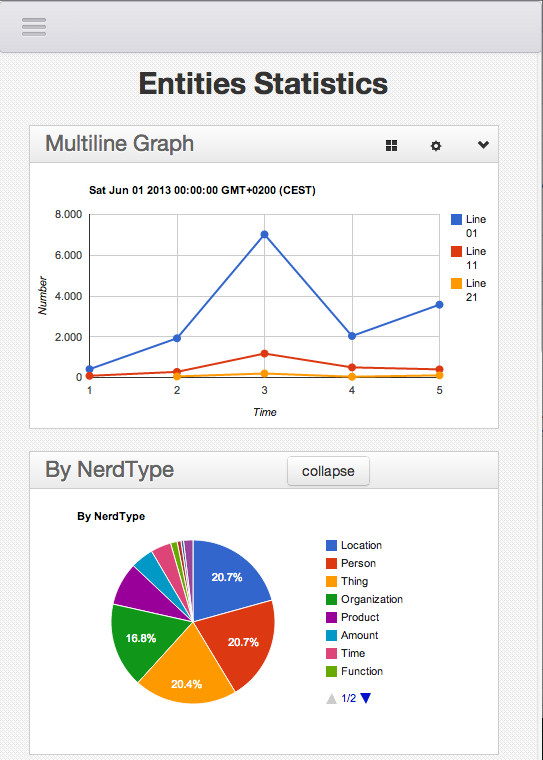
\includegraphics[width=0.4\textwidth]{pics/proto/fullMobile}
\end{figure}
\label{sub:subsection_name}
\chapter{Evaluation} % (fold)
\label{cha:evaluation}
\section{Database issues}
During the deployment the main issues we had to face was database performances issues.
The database is quite large in particular the table entity has more than a million rows. This slowdown the SQL queries and the user interface became not usable: too much latency between the request and the server response.

We localized the problem on the relation entity where the number of rows is higher and especially on group-by operation on nerdType and selection on confidence.


We decided to add indexes to speed up the performance on this queries and we achieved great results.
We created two BTREE INDEX, the first on nerdType and the second on confidence.
\vspace{0.4cm}
        \begin{lstlisting}[language=SQL]
  CREATE INDEX nerdType USING BTREE ON entity(nerdType)
  CREATE INDEX confidence USING BTREE ON entity(confidence); 
        \end{lstlisting}
\vspace{0.9cm}
We now can compare performances on three queries that clearly underline the performance enhance:
\vspace{0.3cm}
        \begin{lstlisting}[language=SQL]
  SELECT nerdType ,
         COUNT(IDENTITY) AS number
  FROM entity AS e,
       annotation AS a
  WHERE e.annotationIdAnnotation = a.idAnnotation
  GROUP BY nerdType
  ORDER BY COUNT(IDENTITY) DESC 
        \end{lstlisting}
\vspace{0.3cm}
This query is executed in 26.66sec without the indexes versus 8.2sec in the second case. The query is more than the 300\% slower with any index.

\vspace{0.9cm}
        \begin{lstlisting}[language=SQL]
   SELECT YEAR(TIMESTAMP) AS YEAR,
         MONTH(TIMESTAMP) AS MONTH,
         DAY(TIMESTAMP) AS DAY,
         COUNT(IDENTITY) AS number
  FROM entity AS e,
       annotation AS a
  WHERE e.annotationIdAnnotation = a.idAnnotation
    AND confidence > "0.99"
  GROUP BY YEAR(TIMESTAMP),
           MONTH(TIMESTAMP),
           DAY(TIMESTAMP) 
        \end{lstlisting}
\vspace{0.3cm}
This query is executed in 3.04sec without the indexes versus 0.66sec in the second case. The query is close to be 500\% slower with any index.

\vspace{0.9cm}
        \begin{lstlisting}[language=SQL]
  SELECT YEAR(TIMESTAMP) AS YEAR,
         MONTH(TIMESTAMP) AS MONTH,
         DAY(TIMESTAMP) AS DAY,
         COUNT(IDENTITY) AS number
  FROM entity AS e,
       annotation AS a
  WHERE e.annotationIdAnnotation = a.idAnnotation
    AND confidence > "0.99"
    AND nerdType = "http://nerd.eurecom.fr/ontology#Person"
  GROUP BY YEAR(TIMESTAMP),
           MONTH(TIMESTAMP),
           DAY(TIMESTAMP) ,
           nerdType
        \end{lstlisting}
\vspace{0.3cm}
This query is executed in 3.4sec without the indexes versus 1.47sec in the second case. The query is more than the 100\% slower with any index.

\chapter{Future work and Conclusions} % (fold)
\label{cha:future_work_and_conclusions}
\section{Future Work}
% chapter future_work_and_conclusions (end)
Although the current development stage is quite advanced some sections are  not yet coded.
Testing is another crucial part we miss to focus on: the application manipulates intensively data and test each module is critically important. Moreover AngularJs offers great feature to create  tests units, allowing to test each service separately (mock services can be injected easily thanks to dependency injection).\newline
Another important aspect is security: the server automatically creates SQL queries taking paramenter that come from the client. At the actual stage of development SQL injection could be exploited to access private data. SQL Injection prevented for the authorization process using methods exposed by the native mySql node.js drivers to escape malicious attack.
This goals could be achieved with few efforts: the problem could be avoided sanitizing the parameters from the users(mySql drivers exposes methods to escape and check for injection attempts).\newline
Last but not least the database performances could slowdown the entire system. The indexes created  will not be enough with the increasing size of the data stored. We have to think about a new structure and relations in our schema to fastly aggregate data for our stats or at least think to create materialized views to speedup performances.\newline
\section{Conclusion}
Every minute Internet generates amount of data that, until some years ago, was even difficult to imagine. Big Data isn't an abstract concept created by some IT guru, but a tangible stream of information that flow throw the network. This data has to be collected and analyzed.Probably the goal of the years that are coming is to create some knowledge from this huge heap of information. Therefore is crucially important to display data in a way that humans can understand it.
\cleardoublepage
\addcontentsline{toc}{chapter}{Bibliography}
\bibliography{biblio}
\end{document}

